% ======================================================= %
%          Phd Thesis of Isis Van Parijs             %
%                                                         %
%  Structure:                                             %
%   template.tex          (main file)                     %
%    - _packages.tex      (load packages)                 %
%    - _settings.tex      (basic configuration)           %
%    - _newcommands.tex   (custom commands)               %
%    - 1 - Introduction/  (chapters in subdirectories)    %
%    - 2 - ...                                            %
%    -                                                    %
%                                                         %
% ======================================================= %

% draft or final?
\newcommand{\status}{draft}
% If the draft option is passed to the package, all micro-typographic extensions will be disabled, which may lead to different line, and hence page, breaks. The draft and final options may also be inherited from the class options; of course, you can override them in the package options. E. g., if you are using the class option draft to show any overfull boxes, you should load microtype with the final option.

% The most general information for this document
\newcommand{\Title}{A search for flavour changing neutral currents involving a top quark and a Z boson, using the data collected by the CMS collaboration at a centre of mass of 13 TeV}
\newcommand{\Pdftitle}{\Title}  % For if you want to have a different title in the pdf document (e.g. special characters removed)
\newcommand{\Author}{Van Parijs, Isis}
\newcommand{\keywords}{LaTeX, template, CMS, FCNC, phd, thesis}
\newcommand{\refereeOne}{Prof.~Dr.~J. D'Hondt}
%\newcommand{\refereeTwo}{Prof.~Dr.~P. Thagoras}
\newcommand{\dateHandIn}{1~June~2017}
\newcommand{\dateDefense}{1~October~2017}


% load the general configuration
%!TEX root = template.tex

% -- packages -------------------------------------- %

% basic layout of the document
\documentclass[
  11pt, a4paper,        % font and paper size
  fleqn,                % align equations to the left
  twoside, openright,   % two sided option with new chapters on the right page
  \status               % the status (defined in main document)
]{memoir}

% general stuff
\usepackage[utf8]{inputenc}   % Input-Encoding
                              % (encoding which is used for saving)
\usepackage[TS1,T1]{fontenc}  % Output-Encoding
                              % (Latin1 [T1] with additional sepecial characters [TS1])

% \usepackage[ngerman]{babel}   % German language package
\usepackage[english]{babel}   % English language package

% image stuff
\usepackage[final]{graphicx}  % include graphics
\usepackage{rotating}         % rotate images
% \usepackage{caption}          % customize your captions (memoir incompatible)
% \usepackage{subfig}           % sub-captions (memoir incompatible, already included there with \subbottom)
\usepackage{wrapfig}          % wrap text around images and tables
\usepackage{afterpage}
\usepackage{lscape}

% font and symbols
\usepackage[charter, greeklowercase=upright]{mathdesign} % Bitstream Charter font, not-italic greek letter like \alphaup
\usepackage[scaled=.96,lining]{XCharter} % Provides additional Charter-like symbols, and small caps
\usepackage{microtype}        % better type setting
% \usepackage{amssymb,amsmath}  % more math symbols and environments % mathdesign interferes with amssymb
% \usepackage{textcomp}         % even more special characters
\usepackage{tikz}             % used to make circled numbers
\usepackage{color}            % define your own colors
\usepackage{scrhack}          % fixes an error caused by listings package
\usepackage{listings}         % enables syntax highlighting for your code
\usepackage{zi4}              % Use Inconsolata for fixed-width texttt

%quotes
%\usepackage{quotchap}

% references
\usepackage[backend=biber,style=numeric-comp]{biblatex}
%\usepackage{cite}
% physics and maths
\usepackage{amsmath}
\usepackage{wasysym}          % glyphs and other symbols, e.g. \int, http://www.ctan.org/pkg/wasysym
\usepackage[alsoload=hep]{siunitx}          % macros for printing numbers (\num{12345}) and units (\SI{1e7}{\kilogram\per\metre\squared}), also interesting: \SIrange{10}{30}{\metre}, \mega\electronvolt, \DeclareSIUnit. \per can be set individually via SI[per-mode=reciprocal], or per-mode-fraction to overwrite the new default in the next line; http://www.ctan.org/pkg/siunitx
\usepackage{commath}          % defines differential operators (\del, \dif)
\usepackage{feynmp-auto}      % Feynman diagrams (alternative: feynmf)
\usepackage{cancel, slashed}  % Feynman notation
% \usepackage{maybemath}        % For context-sensitive maths, like headings
\usepackage{hepparticles}     % particle names
\usepackage{hepnames}         % shortcuts for lots of particle names
\usepackage{braket}           % provides \bra and \ket notation

% configuration
\usepackage{hyperref}         % hyperlinks in PDF
% The two following packages don't work with the memoir style
% \usepackage{fancyhdr}         % configure your page header
% \usepackage[noindentafter]{titlesec}  % configure titles

% table stuff
\usepackage{booktabs}         % professional tables
\usepackage{multirow}         % combine table rows
% \usepackage{arydshln}         % dashed lines in tables

% additional packages (mixed)
% \usepackage{keystroke}        % display keystrokes
\usepackage{xspace}           % adds spaces to the end of commands if needed
\usepackage{pdflscape}        % allows for landscaped, pdf-rotated single pages
\usepackage[acronym,nonumberlist,xindy]{glossaries-prefix}  % glossaries % xindy is used for sorting non-latin characters correctly
\usepackage{multicol}         % offers multi column environments
\usepackage{ifdraft}          % offers \ifdraft{}{} command to do stuff while in draft mode
% \usepackage{panda}            % Custom \panda package for overlining the P
% \usepackage{gitinfo2}         % Provides infos about git (needs hooks, though)

% packages that help during draft versions
% (change document option from draft to final to disable)
\usepackage[obeyDraft,textsize=scriptsize]
  {todonotes}                 % notes and missing images
% \usepackage{showlabels}       % show label names next to numbering

%!TEX root = template.tex

% configure the microtype font setting
\microtypesetup{
  final,        % always activate, even when in draft mode
  activate={true,nocompatibility},  % activate protrusion and expansion
  % tracking=true,  % This is disabled because it adds extra space around small caps. It's suppose to be disabled with \SetTracking{encoding={*}, shape=sc}{0}, but I can't verify this. Maybe you can figure it out!
  kerning=true,
  spacing=true,
  protrusion=true
  % more info on config to be found eg at http://www.khirevich.com/latex/microtype/
}
\microtypecontext{spacing=nonfrench}
% enable protrusion for superscript numbers
% (doesn't work with XeTeX right now)
% \SetProtrusion{
%   encoding={*},
%   family={cmr},
%   series={*},
%   size={6,7}
% }{
%   1={ ,750},2={ ,500},3={ ,500},4={ ,500},5={ ,500},
%   6={ ,500},7={ ,600},8={ ,500},9={ ,500},0={ ,500}
% }


% until where should titles be enumerated?
\setsecnumdepth{subsubsection}
\settocdepth{subsection}


% size parameters
\setlength{\textwidth}{150mm}       % width of the text area
\setlength{\textheight}{220mm}      % height of the text area
\setlength{\hoffset}{0pt}           % offset insertet at the left
\setlength{\voffset}{10pt}          % offset inserted at the top
\setlength{\oddsidemargin}{9mm}     % offset inserted to the left for odd pages
\setlength{\evensidemargin}{0mm}    % offset inserted to the left for even pages
\setlength{\marginparwidth}{18mm}   % width for marginal notes (Randnotizen)
\setlength{\parskip}{\bigskipamount} % space between two paragraphs
\setlength{\parindent}{10pt}        % indention for a new paragraph


% colors
\definecolor{gray75}{gray}{0.75}
\definecolor{gray90}{gray}{0.90}
\definecolor{darkblue}{rgb}{0,0,0.5}
\definecolor{darkgreen}{rgb}{0,0.5,0}
\definecolor{green}{rgb}{0.2,0.8,0.2}
\definecolor{red}{rgb}{1.0,0.3,0.0}
\definecolor{orange}{rgb}{1.0,0.6,0.0}


% some PDF settings (like hyperlinks in color)
\hypersetup{
 % pdftex,                   % use pdftex backend
 pdfencoding=auto,         % encoding
 pdftitle={\Pdftitle},     % title
 pdfauthor={\Author},      % author
 bookmarksnumbered=true,   % put section numbers in bookmarks
 % linktocpage=true,         % make page number (not text) be link on TOC
 % pdfpagelabels=true,       % set PDF page labels
 colorlinks=true,          % false: boxed links; true: colored links
 linkcolor=darkblue,       % color of internal links
 citecolor=darkblue,       % color of links to bibliography
 filecolor=darkblue,       % color of file links
 urlcolor=darkblue,        % color of external links
 draft=false               % always show links, even in draft mode
}

% settings for siunitx, see http://www.ctan.org/pkg/siunitx
\sisetup{
  per-mode = symbol,       % creates a backslash for division as default, can be overridden individually
  separate-uncertainty = true,  % dont use "10.0(1)" notation for uncertainties, but do use "10.0 \pm 0.1"
  binary-units = true,      % load also binary units like bit/byte
  list-final-separator = {, and~}  % use Oxford comma for \SIlist-s
}


% chapter definition
\newif\ifchapternonum
\makechapterstyle{jenor}{
  \renewcommand\printchaptername{}
  \renewcommand\printchapternum{}
  \renewcommand\printchapternonum{\chapternonumtrue}
  \renewcommand\chaptitlefont{\fontseries{bx}%
    \fontshape{n}\fontsize{25}{35}\selectfont\raggedleft}
  \renewcommand\chapnumfont{\fontseries{m}\fontshape{n}%
    \fontsize{3cm}{0in}\selectfont\color{gray75}}
  \renewcommand\printchaptertitle[1]{%
    \noindent%
    \ifchapternonum%
    \begin{tabularx}{\textwidth}{X}%
      {\parbox[b]{\linewidth}{\chaptitlefont ##1}%
      \vphantom{\raisebox{-15pt}{\chapnumfont 1}}}
    \end{tabularx}%
    \else
    \begin{tabularx}{\textwidth}{Xl}
      {\parbox[b]{\linewidth}{\chaptitlefont ##1}}
      & \raisebox{-15pt}{\chapnumfont\ \thechapter}%
    \end{tabularx}%
    \fi
    \par\vskip2mm\hrule
  }
}
\chapterstyle{jenor}


% other title definitions
% change the following to switch to sans serif title styles
% \setsecheadstyle{\fontfamily{\sfdefault}\Large\bfseries}
% \setsubsecheadstyle{\fontfamily{\sfdefault}\large\bfseries}
% \setsubsubsecheadstyle{\fontfamily{\sfdefault}\bfseries}
% \setparaheadstyle{\fontfamily{\sfdefault}\bfseries}
% \setsubparaheadstyle{\fontfamily{\sfdefault}\bfseries}


% table of contents
% \renewcommand{\cftsectionfont}{\fontfamily{\sfdefault}\selectfont\small}
% \renewcommand{\cftsubsectionfont}{\fontfamily{\sfdefault}\selectfont\small}


% caption styling
\captiontitlefont{\small}
\captionnamefont{\small\bfseries}
\indentcaption{10pt}

% Subfloats for figures (memoir option)
\newsubfloat{figure}

% rotate labels from showlabels to make them fit on the margin
% \renewcommand{\showlabelfont}{\scriptsize\ttfamily}
% \renewcommand{\showlabelsetlabel}[1]{\begin{turn}{60}\showlabelfont #1\end{turn}}


% Bibliography options
% \bibliographystyle{custom}

% Glossaries options
\renewcommand*{\glspostdescription}{}  % redefine the character displayed after an glossary entry from dot to nothing
\makeglossaries  % ensure glossary files are created
\glstoctrue  % Put glossaries into TOC
% to change the title of your acronyms uncomment the following lines and the correspoinding \makeglossaries in the main document
 %\providecommand{\myacronymtitle}{List of Acronyms}

% Makes the header not italics
\makeevenhead{headings}{\thepage}{}{\leftmark}
\makeoddhead{headings}{\rightmark}{}{\thepage}

% Customize todonotes
% First, get rid of the rounded corners
\makeatletter
\tikzstyle{notestyleraw} = [
draw=\@todonotes@currentbordercolor,
fill=\@todonotes@currentbackgroundcolor,
line width=0.5pt,
text width = \@todonotes@textwidth - 1.6 ex - 1pt,
inner sep = 0.8 ex,
rounded corners=0pt]
\makeatother
% Second, change default colors
\presetkeys{todonotes}{backgroundcolor=brightorange, bordercolor=orange,
prepend, caption={\textbf{\textcolor{darkorange}{NOTE}}}}{}




%!TEX root = template.tex

% fancy header



% general commands
\renewcommand{\>}{\frqq}
\newcommand{\<}{\flqq}
\newcommand{\myquote}[1]{\frqq{}#1\flqq{}\xspace}
\newcommand{\mysinglequote}[1]{\frq#1\flq{}\xspace}

% shortcuts for references
\newcommand{\fig}[1]{\hyperref[#1]{Figure \ref*{#1}}}
\newcommand{\tab}[1]{\hyperref[#1]{Table \ref*{#1}}}
\newcommand{\eq}[1]{\hyperref[#1]{Equation \ref*{#1}}}
\newcommand{\Sec}[1]{\hyperref[#1]{Section \ref*{#1}}}

% circled numbers
\newcommand*\circled[1]{\tikz[baseline=(char.base)]{
            \node[shape=circle,draw,inner sep=1.5pt] (char) {#1};}}

% citation needed
\newcommand{\todocite}[0]{\todo[color=green!40]{Add source}}


%abbreviations
\newcommand{\SM}{SM}
\newcommand{\BSM}{BSM}
\newcommand{\pu}{pileup}
% useful commands for equations
\newcommand{\e}{\enspace}  % width of one digit
\newcommand{\dd}{\,\mathrm{d}}
% \newcommand{\del}{\partial}  % comes from package commath
\newcommand{\Ra}{\Rightarrow}
\newcommand{\ra}{\rightarrow}

%\renewcommand{\vec}[1]{\underline{#1}}
\newcommand{\heq}{\widehat{=}}
\renewcommand{\deg}{$\,^\circ$}
\newcommand{\chindof}{\chi^2/\mathrm{ndof}}
\newcommand{\com}{$\sqrt{s}$ }
\newcommand{\impuls}{$\vec{p}$ }
\newcommand{\trimpuls}{\ensuremath{\vec{p}_{\mathrm{T}}} }
\newcommand{\pt}{\ensuremath{p_{\mathrm{T}}} }
\newcommand{\ptmisvec}{\ensuremath{\vec{p}_{\mathrm{T}}^{\mathrm{miss}}} }
\newcommand{\ptmis}{\ensuremath{p_{\mathrm{T}}^{\mathrm{miss}}} }
\newcommand{\Etmis}{\ensuremath{E_{\mathrm{T}}^{\mathrm{miss}}} }
\newcommand{\Et}{\ensuremath{E_{\mathrm{T}}} }
\newcommand{\psrap}{$\eta$ }
\newcommand{\abspsrap}{\ensuremath{\left| \eta\right|} }
\newcommand{\GeVinv}{\ensuremath{\GeV^{-1}}}
\newcommand{\xcal}[1]{\text{\usefont{OMS}{cmsy}{m}{n}#1}}  % Use original mathcal font instead of charters mathcal version
\newcommand{\orderof}[1]{$\xcal{O}\left( #1 \right)$}  % \orderof{\si{\metre}} now is more beautiful
\newcommand{\BR}{\ensuremath{\mathcal{B}}\xspace}
\newcommand{\FCNC}{FCNC}
% new units for siunitx package
\newcommand{\qe}{\ensuremath{q_{\mathrm{e}}}\xspace}

\DeclareSIUnit\event{ev}
\DeclareSIUnit\channel{ch}
\DeclareSIUnit\MeV{MeV}
\DeclareSIUnit\GeV{GeV}
\DeclareSIUnit\TeV{TeV}
\DeclareSIUnit\Tesla{T}
\DeclareSIUnit{\atm}{atm}
\DeclareSIUnit{\ADC}{ADC}
\DeclareSIUnit{\pb}{pb}
% particles
\newcommand{\NPL}{\ensuremath{\mathrm{NPL}}}
\newcommand{\muR}{\ensuremath{\mu_{\mathrm{R}}}}
\newcommand{\muF}{\ensuremath{\mu_{\mathrm{F}}}}
\newcommand{\accept}{\ensuremath{\mathfrak{A}}}
\newcommand{\st}{single top}
\renewcommand{\tt}{top pair }
\newcommand{\Lagr}{\ensuremath{\mathcal{L}}}
\newcommand{\lagr}{\ensuremath{\mathcal{L}}}
\newcommand{\like}{\ensuremath{\mathfrak{L}}}
\newcommand{\lumi}{\ensuremath{\mathrm{L}}}
\newcommand{\SSU}{\ensuremath{\mathrm{SU}_{\mathrm{C}}(3) \times \mathrm{SU}_{\mathrm{L}}(2) \times \mathrm{U}_{\mathrm{Y}}(1)}}
\newcommand{\Uone}{\ensuremath{\mathrm{U}_{\mathrm{Y}}(1)}}
\newcommand{\SU}{\ensuremath{\mathrm{SU}_{\mathrm{L}}(2) \times \mathrm{U}_{\mathrm{Y}}(1)}}
\newcommand{\Sthree}{\ensuremath{\mathrm{SU}_{\mathrm{C}}(3)}}
\newcommand{\Stwo}{\ensuremath{ \mathrm{SU}_{\mathrm{L}}(2)}}
\newcommand{\Bfield}{\ensuremath{ \mathrm{B}_{\mu}}}
\newcommand{\Wfieldone}{\ensuremath{ \mathrm{W}_{\mu}^1}}
\newcommand{\Wfieldtwo}{\ensuremath{ \mathrm{W}_{\mu}^2}}
\newcommand{\Wfieldthree}{\ensuremath{ \mathrm{W}_{\mu}^3}}
\newcommand{\Gfields}{\ensuremath{ \mathrm{G}_{\mu}^{1...8}}}
\newcommand{\Gtensord}{\ensuremath{ \mathrm{G}_{\mu\nu}^{i}}}
\newcommand{\Gtensor}{\ensuremath{ \mathrm{G}_{\mu\nu}}}
\newcommand{\Ztensor}{\ensuremath{ \mathrm{Z}_{\mu\nu}}}
\newcommand{\Gtensoru}{\ensuremath{ \mathrm{G}^{\mu\nu i}}}
\newcommand{\Wtensord}{\ensuremath{ \mathrm{W}_{\mu\nu}^{i}}}
\newcommand{\Wtensoru}{\ensuremath{ \mathrm{W}^{\mu\nu i}}}
\newcommand{\Btensord}{\ensuremath{ \mathrm{B}_{\mu\nu}^{i}}}
\newcommand{\Btensoru}{\ensuremath{ \mathrm{B}^{\mu\nu i}}}
\newcommand{\photonfield}{\ensuremath{ \mathrm{A}_{\mu}}}
\newcommand{\photontensor}{\ensuremath{ \mathrm{A}_{\mu\nu}}}
\newcommand{\Zfield}{\ensuremath{ \mathrm{Z}^0_{\mu}}}
\newcommand{\Wfield}{\ensuremath{ \mathrm{W}_{\mu}^{\pm}}}
\newcommand{\sW}{\ensuremath{\mathrm{sin } \theta_{\mathrm{W}}}}
\newcommand{\cW}{\ensuremath{\mathrm{cos } \theta_{\mathrm{W}}}}
\newcommand{\mtw}{\ensuremath{m_{\mathrm{T}}(\W)}\xspace}
\newcommand{\mZ}{\ensuremath{m_{\mathrm{Z}}}\xspace}
\newcommand{\LSM}{\ensuremath{\Lagr_\mathrm{SM}}}
\DeclareRobustCommand{\order}{\ensuremath{\mathcal{O}}}
\newcommand{\tZq}{\ensuremath{\mathrm{tZ}\Pquark}}
\newcommand{\kgqt}{\ensuremath{\kappa_{\Pgluon\Pquark\Ptop}}}
\newcommand{\kZqt}{\ensuremath{\kappa_{\Ptop\PZ\Pquark}}}
\newcommand{\eHqt}{\ensuremath{\eta_{\Ptop\PHiggs\Pquark}}}
\newcommand{\kfqt}{\ensuremath{\kappa_{\Ptop\Pphoton\Pquark}}}
\newcommand{\kgqtl}{\ensuremath{\kappa_{\Pgluon\Pquark\Ptop}/\Lambda}}
\newcommand{\kZqtl}{\ensuremath{\kappa_{\Ptop\PZ\Pquark}/\Lambda}}
\newcommand{\kfqtl}{\ensuremath{\kappa_{\Ptop\Pphoton\Pquark}/\Lambda}}
\newcommand{\zZqt}{\ensuremath{\zeta_{\mathrm{\Ptop\PZ\Pquark}}}\xspace}
\newcommand{\zZut}{\ensuremath{\zeta_{\mathrm{\Ptop\PZ\Pup}}}\xspace}
\newcommand{\zZct}{\ensuremath{\zeta_{\mathrm{\Ptop\PZ\Pcharm}}}\xspace} 
\newcommand{\zWqt}{\ensuremath{\zeta_{\mathrm{\Ptop\PW\Pquark}}}\xspace} 
\newcommand{\antikt}{\ensuremath{\mathrm{anti-k}_{\mathrm{T}}}}
\newcommand{\dbeta}{\ensuremath{\Delta\beta}}
\newcommand{\iso}{\ensuremath{\mathcal{I} }}
\newcommand{\kxqt}{\ensuremath{\kappa_{\Ptop \mathrm{X} \Pquark}}/\Lambda\xspace}
\newcommand*\textfrac[2]{              % display fraction in textstyle
	\frac{\text{#1}}{\text{#2}}
}

\newenvironment{chapquote}[2][2em]
{\setlength{\@tempdima}{#1}%
	\def\chapquote@author{#2}%
	\parshape 1 \@tempdima \dimexpr\textwidth-2\@tempdima\relax%
	\itshape}
{\par\normalfont\hfill--\ \chapquote@author\hspace*{\@tempdima}\par\bigskip}


% particles
\renewcommand{\Pquark}{\ensuremath{\mathrm{q}}}
\renewcommand{\APquark}{\ensuremath{\bar{\mathrm{q}}}}
\renewcommand{\Pup}{\ensuremath{\mathrm{u}}}
\renewcommand{\APup}{\ensuremath{\bar{\mathrm{u}}}}
\renewcommand{\Pdown}{\ensuremath{\mathrm{d}}}
\renewcommand{\APdown}{\ensuremath{\bar{\mathrm{d}}}}
\renewcommand{\Pbottom}{\ensuremath{\mathrm{b}}}
\renewcommand{\APbottom}{\ensuremath{\bar{\mathrm{b}}}}
\renewcommand{\Ptop}{\ensuremath{\mathrm{t}}}
\renewcommand{\APtop}{\ensuremath{\bar{\mathrm{t}}}}
\newcommand{\ttbar}{\ensuremath{\mathrm{t}\bar{\mathrm{t}}}}
\newcommand{\qqbar}{\ensuremath{\mathrm{q}\bar{\mathrm{q}}}}
\newcommand{\tZ}{\ensuremath{\mathrm{tZ}}}
\newcommand{\tbarZ}{\ensuremath{\bar{\mathrm{t}}\mathrm{Z}}}
\newcommand{\bbbar}{\ensuremath{\mathrm{b}\bar{\mathrm{b}}}}
\newcommand{\ttZ}{\ensuremath{\ttbar\mathrm{Z}}}
\newcommand{\ttW}{\ensuremath{\ttbar\mathrm{W}}}
\newcommand{\ttH}{\ensuremath{\ttbar\mathrm{H}}}
\newcommand{\WZ}{\ensuremath{\mathrm{WZ}}}
\newcommand{\WZZ}{\ensuremath{\mathrm{WZZ}}}
\newcommand{\WW}{\ensuremath{\mathrm{WW}}}
\newcommand{\WWZ}{\ensuremath{\mathrm{WWZ}}}
\newcommand{\ZZ}{\ensuremath{\mathrm{ZZ}}}
\newcommand{\ZZZ}{\ensuremath{\mathrm{ZZZ}}}
\newcommand{\tWZ}{\ensuremath{\mathrm{tWZ}}}
\newcommand{\tqH}{\ensuremath{\mathrm{tqH}}}
\newcommand{\DY}{\ensuremath{\PZ/\Pgammastar+\mathrm{jets}}}
% Software
\newcommand{\Geant}{\texttt{Geant}}
\newcommand{\aMCMG}{\texttt{MadGraph5$\_$aMC$@$NLO}}
\newcommand{\MG}{\texttt{MadGraph}}
\newcommand{\aMC}{\texttt{aMC$@$NLO}}
\newcommand{\Powheg}{\texttt{POWHEG}}
\newcommand{\MS}{\texttt{MadSpin}}
\newcommand{\Pythia}{\texttt{Pythia}}
\newcommand{\FR}{\texttt{FeynRules}}
\newcommand{\UFO}{\texttt{Universal Feynrules Output}}
\newcommand{\CTEQ}{\texttt{CTEQ}}
\newcommand{\JHU}{\texttt{JHU}}
\newcommand{\ME}{\texttt{MadEvent}}

%\addbibresource{references.bib}  % Use with BibLaTeX
\addbibresource{Bibliography/Chapter2.bib}
\addbibresource{Bibliography/CMS.bib}

% -------------------------------------------------- %
%    title, TOC, ...                                 %
% -------------------------------------------------- %

% begin the document
\begin{document}
\frontmatter

%%!TEX root = template.tex

%\newglossaryentry{gls:template}{
%    name = {this template},
%    description = {This awesomely great template thing}
%}
%\newacronym{jama}{JAMA}{Just A Meaningless Acronym}
%\newacronym[prefixfirst={the~}]{aalf}{AALF}{Arms And Legs Facility}

%\newacronym{hcal}{HCAL}{hadronic calorimeter}
\newglossaryentry{gls:hcal}{
    name = {HCAL},
    description = {Hadroni calorimeter}
}

% the title page
%!TEX root = template.tex

% \begin{titlepage}
\begin{center}
	\vspace*{5mm}
     
    \begin{figure}[ht]
    	\centering
    	\includegraphics[width=0.5\linewidth]{"VUB MONO positief/VUB MONO POSITIEF OUTLINE"}
    %	\caption{}
    	\label{fig:vub-mono-positief-outline}
    \end{figure}
    
	\huge \textbf{\Title}

	\vspace{10mm}

	\Large \Author
	
	\vspace{15mm}
	\large \textbf{Proefschrift ingediend met het oog op het behalen van de academische graad Doctor in de Wetenschappen.}

	\vspace{25mm}
	\small
	\begin{tabular}{rl}
     Published in & Faculteit Wetenschappen \& Bio-ingenieurswetenschappen \\[2mm]
                  &\large Vrije Universiteit Brussel \\[2mm]
%                  & Departement ELEM \\ [2mm]
 %           Issue & \large 18e9 Rev. 7 \emph{Cataclysm} \\[2mm]
               At & \large 10 November 2017.\\[15mm]
   Responsible Contact: & \large Isis Van Parijs \\[1mm]
                  & Interuniversitary Intitute for High Energy Physics\\
                  Supervisor: & Prof. Jorgen D'Hondt
	\end{tabular}


\end{center}
% \end{titlepage}

\thispagestyle{empty}
\newpage
\null

Doctoral examination commission:\\

\begin{tabular}{l l @{\hspace{1cm}} l l}
	Chair:& & Prof. Dr. B. Craps & Vrije Universiteit Brussel \\
	Supervisor: && Prof. Dr. J. D'Hondt & Vrije Universiteit Brussel \\ 
	Secretary:& & Prof. Dr. S. Buitink & Vrije Universiteit Brussel \\
	Other:& & & \\
	&DNTK: & Prof. Dr. P. Van Mulders & Vrije Universiteit Brussel  \\
	&DSCH: & Prof. Dr. S. Ballet & Vrije Universiteit Brussel  \\
	&External & Prof. Dr. B. Fuks  & University Pierre and Marie Curie (Paris VI) \\
	&External: & Prof. Dr. A. Onofre & LIP and University do Minho 
\end{tabular}


\vfill
\begin{tabular}{l @{\hspace{1cm}} l l}
	Date of Hand-in: & \dateHandIn &\\
	Date of Private Defense: & \dateDefense &
\end{tabular}
\vspace{10mm}

\textcopyright\ 2017 Isis Van Parijs\\
All rights reserved. No parts of this book may be reproduced or transmitted in any form or by any means, electronic, mechanical, photocopying, recording, or otherwise, without the prior written permission of the author.
% \newpage
% \thispagestyle{empty}
% \mbox{}
\cleardoublepage{}

\setlength{\topmargin}{0mm}
\normalsize%\rm


% table of contents
%Protrusion (margin kerning, hanging punctuation) enables characters to cross the margin edge in order to increase uniformity of the optical appearance of text boundaries (see pages 39–50 of Hàn Thế Thành’s dissertation). After activating protrusion with the option activate={true,nocompatibility} of microtype, crossing the margins is best seen for the characters having small area (".", ",", "-") or highly non-flat contour near the margin edge ("y", "r" near the right margin). This is illustrated in the figure below where comma and "r" cross the right margin edge indicated by the red dashed line:
\microtypesetup{protrusion=false} % disables protrusion locally in the document
\tableofcontents*
\microtypesetup{protrusion=true}  % enables protrusion again
\newpage

% load glossaries

% -------------------------------------------------- %
%    the main content                                %
% -------------------------------------------------- %

\mainmatter
\chapter[An introduction to the theory]{Theoretical bases}
%Disentangling Heavy Flavor at Colliders
% https://arxiv.org/abs/1702.02947

%Why dim 6 operators? 
%https://indico.cern.ch/event/610458/#4-top-16-017-eft-re-interpreta

%EFT Theory
%https://indico.cern.ch/event/537012/timetable/#day-2016-11-23
%https://indico.cern.ch/event/612805/

%eft interpretation 
% https://mail.google.com/mail/u/0/?tab=wm#inbox/15b57592ac482483
% https://twiki.cern.ch/twiki/bin/view/CMS/TopEFT
\section{Elementary particles and forces}
\section{Standard Model Lagrangian}
\section{Physics beyond the standard model}
\subsection{Effective field theory}
\subsection{Motivations for new physics}
\subsection{Searches beyond the Standard Model}
\subsection{Experimental and theoretical constraints}
\section{Statistics for a high energy particle physiscist}
\subsection{Boosted decision trees}
\subsection{Confidence levels }
\subsection{Combine limit setting tool}

\chapter{Experimental setup}
%\epigraph{The LHC rose from the dead on Easter. I've heard thats been done before... There is a place in human knowledge where here be dragons. That is the place where the ship that is the LHC  will be going.}
%	{\textit{Don Lincoln, tedX}}


A key objective of the Large Hadron Collider (LHC) was the search for the Brout-Englert-Higgs boson. The Large  Electron Positron (LEP)~\cite{Myers:226776} and Tevatron~\cite{1748-0221-6-08-T08001} experiments established that the mass of the scalar boson has to be larger than 114 \GeV~\cite{Barate:2003sz,Herner:2016woc}, and smaller than approximate 1 \TeV\ due to unitarity and perturbativity constraints~\cite{Djouadi:2005gi}. On top of this, the search for new physics such as supersymmetry or the understanding of dark matter were part of the motivation for building the LHC. 
Since the start of its operation, the LHC is pushing the boundaries of the Standard Model, putting the most stringent limits on physics beyond the Standard Model as well as precision measurements of the parameters of the Standard Model. A milestone of the LHC is the discovery of the scalar boson in 2012 by the two largest experiments at the LHC~\cite{Chatrchyan:2012xdj,Aad:2012tfa}.

This chapter is dedicated to the experimental set-up of the LHC and the Compact  Muon Solenoid (CMS) experiment. \Sec{sec:LHC} describes the LHC and its acceleration process for protons to reach their design energies. The CMS experiment and its components are presented in \Sec{sec:CMS}. The upgrades performed during the long shutdown in 2013 are discussed in \Sec{sec:Phase1}. The data acquisition of CMS is presented in \Sec{sec:DAQ}, while the CMS computing model is shown in \Sec{sec:Computing}.


\section{The Large Hadron Collider}
\label{sec:LHC}
The LHC has started its era of cutting edge science on 10 September 2008~\cite{LHC:2008} after approval by the European Organisation of Nuclear Research (CERN) in 1995~\cite{Pettersson:291782}. Installed in the previous LEP tunnel, the LHC consists of a 26.7~\km\ quasi ring, that is installed between 45 and 170~\m\ under the French-Swiss border amidst Cessy (France) and Meyrin (Switzerland). Built to study rare physics phenomena at high energies, the LHC  can accelerate mainly two types of particles, protons and lead ions Pb$^{45+}$, and provides collisions at four interaction points, where the particle bunches are crossing. Experiments for studying the collisions are installed at each interaction point. 

 As can be seen in \fig{fig:LHCchain}, the LHC is the last element in a chain that creates, injects and accelerates protons. The starting point is the ionisation of hydrogen, creating protons that are injected in a linear accelerator (LINAC 2). Here, the protons obtain an energy of 50~\MeV. They continue to the Proton Synchrotron Booster (PSB or Booster), where the packs of protons are accelerated to 1.4~\GeV\ and each pack is split up in twelve bunches with 25 or 50~\nano\s\ spacing. The Proton Synchrotron (PS) then increases their energy to 25~\GeV\ before the Super Proton Synchrotron (SPS) increases the proton energy up to 450~\GeV. Each accelerator ring expands in radius in order to reduce the energy loss of the protons by synchrotron radiation\footnote{This energy loss is proportional to the fourth power of the proton energy and inversely proportional to the bending radius.}. Furthermore, the magnets responsible for the bending of the proton trajectories have to be strong enough to sustain the higher proton energy. Ultimately, the proton bunches are injected into opposite directions into the LHC, where they are accelerated to 3.5 \TeV\ (in 2010 and 2011), 4~\TeV\ (in 2012 and 2013) or 6.5~\TeV\ (in 2015 and 2016)~\cite{Wenninger:2254678}. 
  \begin{figure}[h]
 	\centering
 	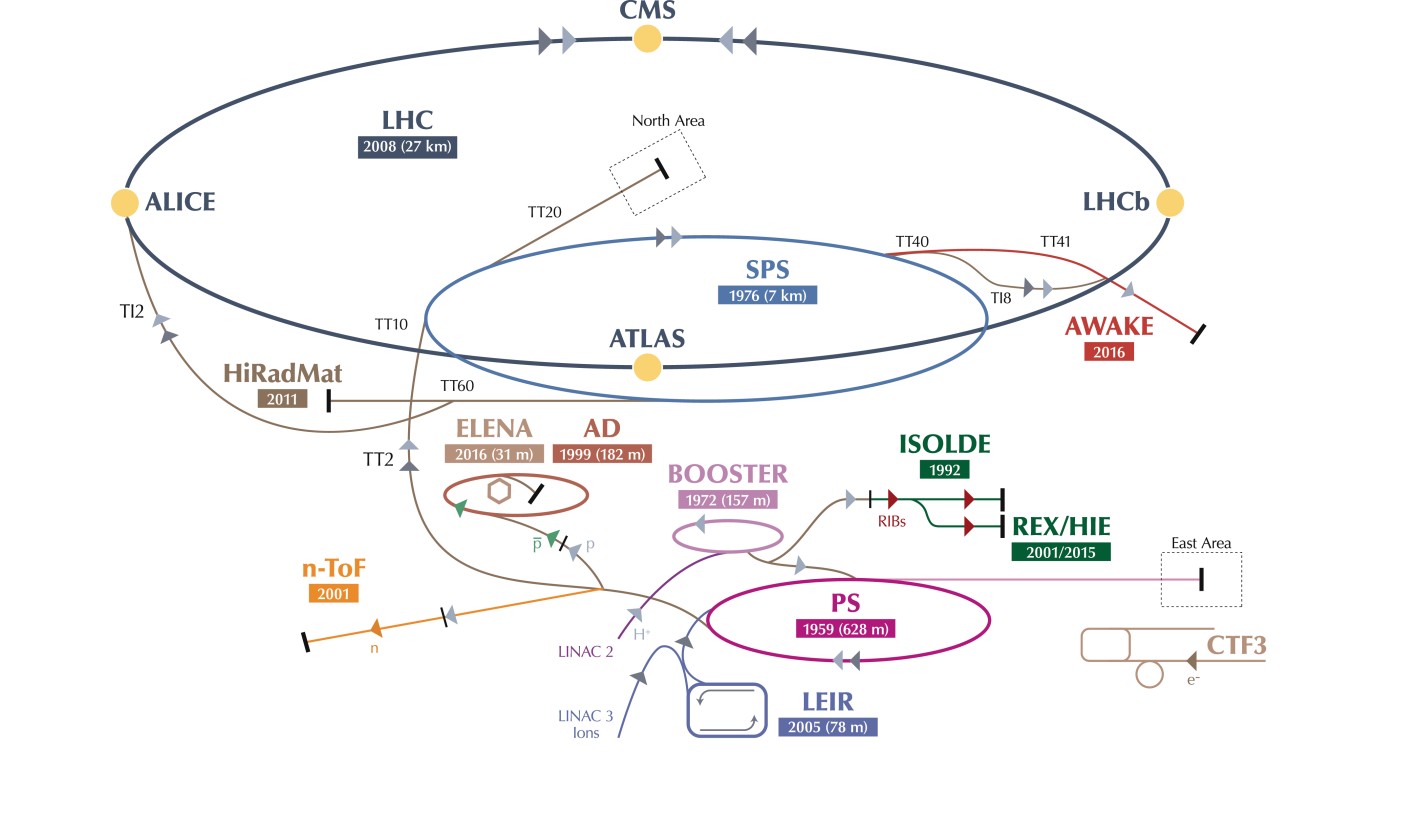
\includegraphics[width=1.\textwidth]{2_ExperimentalSetup/Figures/CCC-v2016}
 	\caption{Schematic representation of the accelerator complex at CERN~\cite{DeMelis:2197559}. The LHC (dark blue) is the last element in chain of accelerators. Protons are successively accelerated by LINAC 2, the Booster, the Proton Synchrotron (PS) and the Super Proton Synchrotron (SPS) before entering the LHC.}
 	\label{fig:LHCchain}
 \end{figure}

In \fig{fig:lhcschedule} the LHC programme is shown. the first data collisions, so-called Run 1 period, lasted from 2008 until 16 February 2013 after which  the CERN accelerator complex shut down for two years of planned maintenance and consolidation during so-called long shutdown 1 (LS1). On 23 March 2015, the new data taking period known as Run 2 started. With a brief end of the year extended technical stop (EYETS). The main activities carried out during the EYETS were the maintenance of systems such as the cryogenics, the cooling, electrical systems, etc.; the replacement of the magnet, as well as a de-cabling and cabling campaign on the SPS\cite{MurilloQuijada:2017agx}. Run 2 will last until July 2018 when the  long shutdown 2 (LS2) will begin for 2 years. The main goal of this shutdown is the LHC injectors upgrade (LUI), but also maintenance and consolidation will be performed. Furthermore, preparations for the High Luminosity LHC, which will start in 2024, will be done. More information about phase 1 upgrades during LS1 and EYETS is given in \Sec{sec:Phase1}.\\ %https://home.cern/cern-people/updates/2017/01/eyets-report-so-far-so-good\
 Before the start of the LHC in 2010, the previous energy record was held by the Tevatron collider at Fermilab, colliding protons with antiprotons at \com = 1.96~\TeV.  When completely filled, the LHC nominally contains 2220 bunches in Run 2, compared to 1380 in Run 1 (design: 2200). 
%At full intensity, it would have nearly 2800 bunches but this is limited due to a problem with SPS in 2016.
\begin{figure}[htbp]
	\centering
	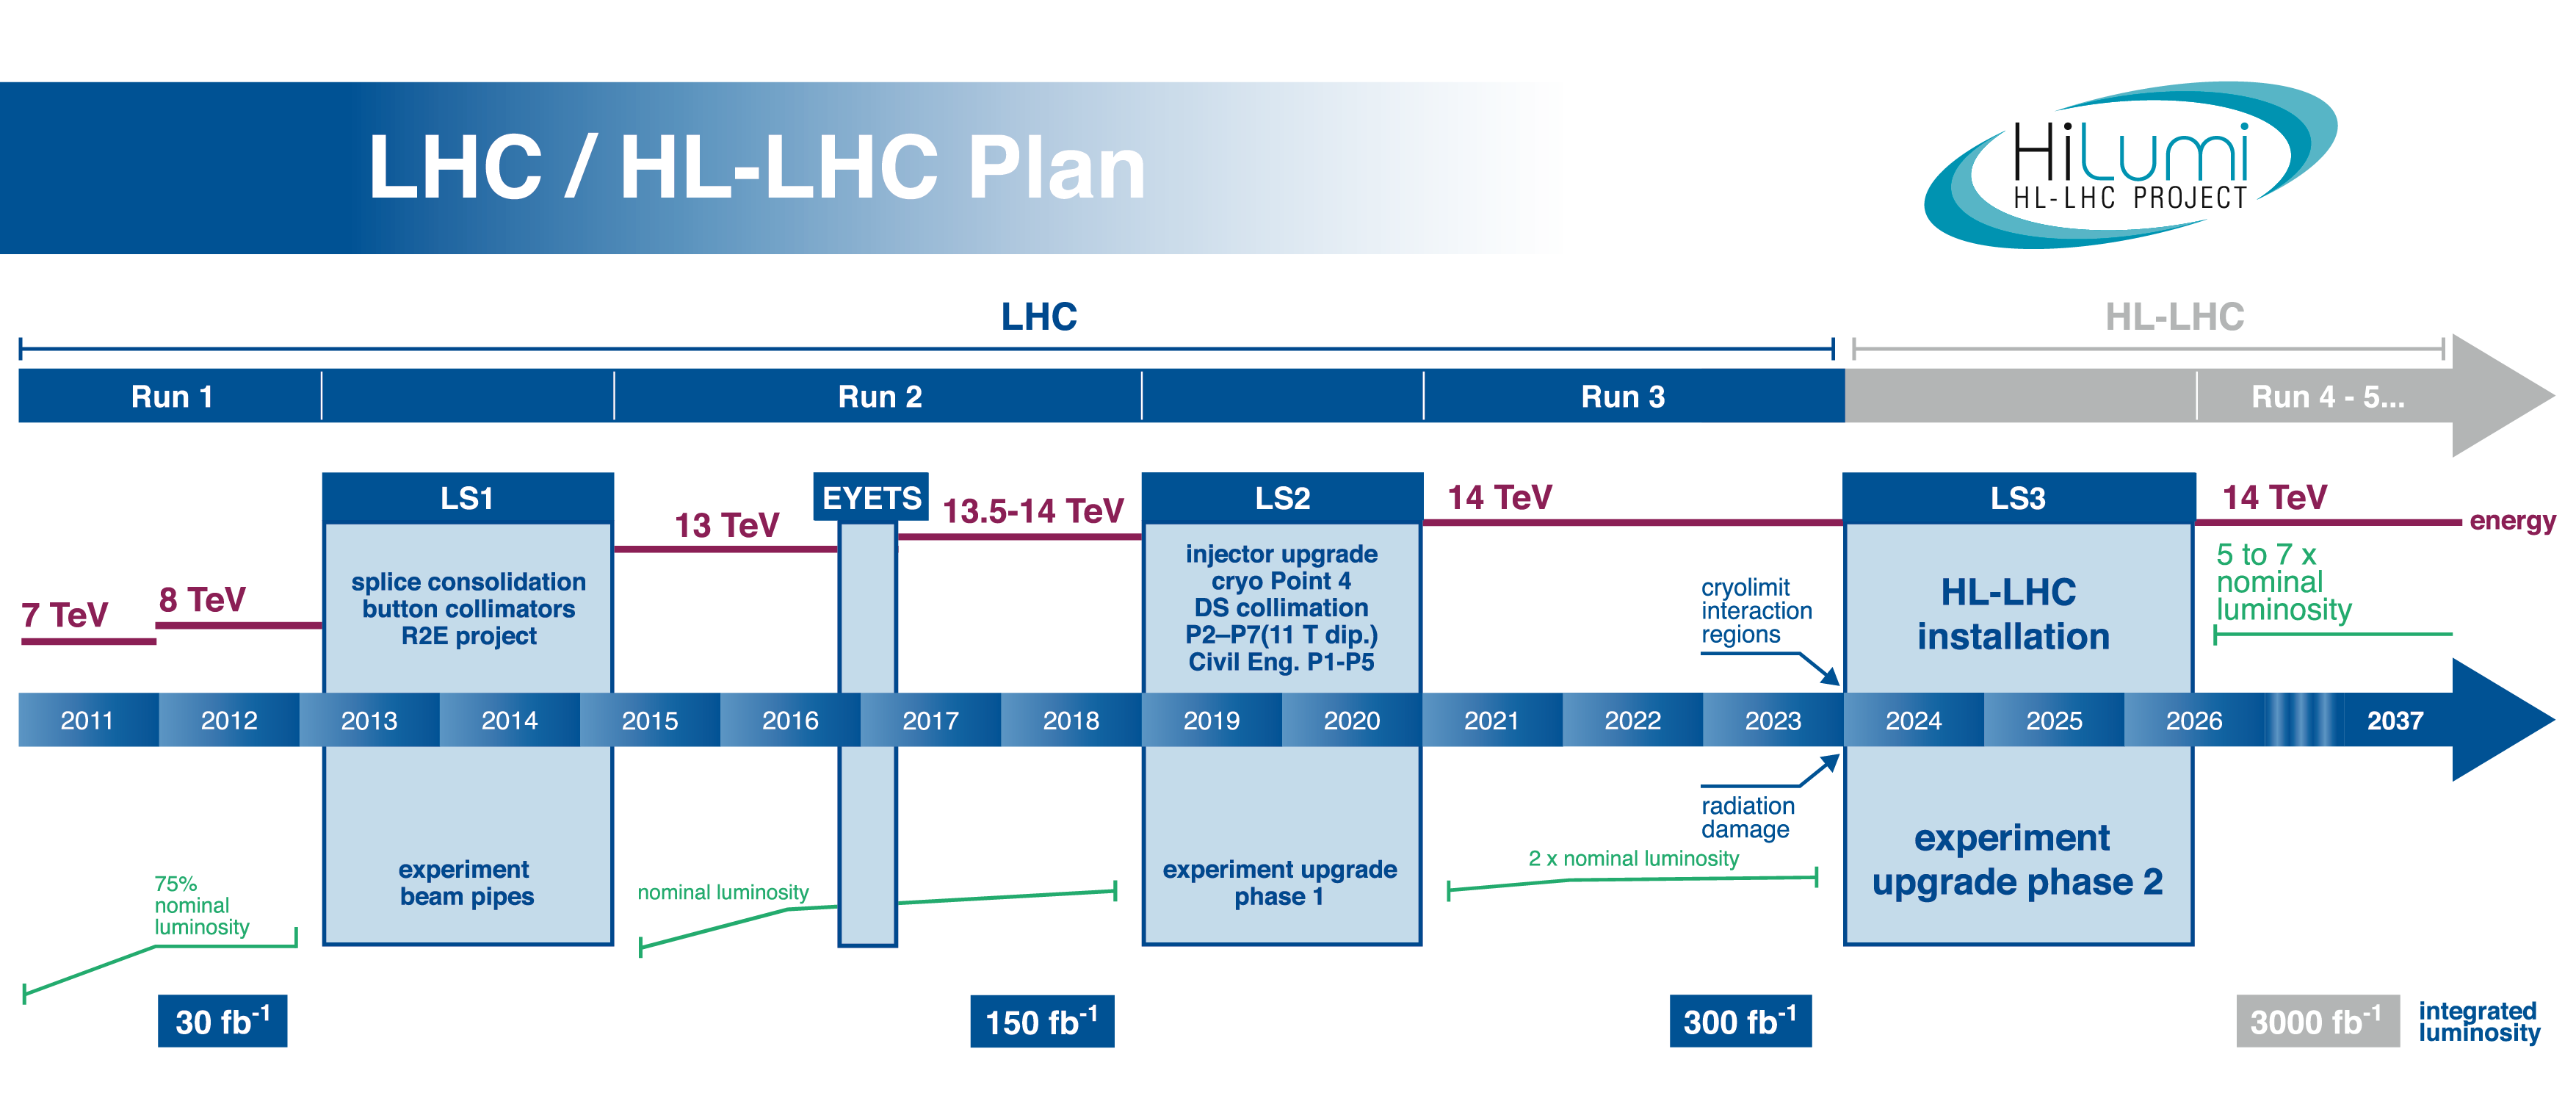
\includegraphics[width=1.\linewidth]{2_ExperimentalSetup/Figures/lhc_schedule}
	\caption{The HL-LHC timeline. Figure taken from \cite{Antonella:1975962}.}
	\label{fig:lhcschedule}
\end{figure}


Inside the LHC ring~\cite{Bruning:782076}, the protons are accelerated by the means of radio frequency cavities, while 1232 dipole magnets of approximately 15~\m\ long, each weighing 35~\tonne\, ensure the deflection of the beams.  The two proton beams circulate in opposite direction in separate pipes inside of the magnet. Through the use of a strong electric current in the coils of the magnet, magnetic fields are generated and cause the protons to bend in the required orbits. In order for the coil to become superconducting and able to produce a strong magnetic field of 8.3~\tesla, the magnet structure is surrounded by a vessel. This vessel is filled with liquid Helium making it possible to cool down the magnet to 1.9~\kelvin. In order to get more focussed and stabilised proton beams, additional higher-order multipole and corrector magnets are placed along the LHC beam line.

  

The LHC is home to seven experiments, each located at an interaction point: 
\begin{itemize}
	\item A Toroidal LHC ApparatuS (ATLAS)~\cite{Aad:2008zzm} and the Compact Muon Solenoid (CMS)~\cite{Chatrchyan:2008aa} experiments are the two general purpose detectors at the LHC. They both have a hermetic, cylindrical structure and were designed to search for new physics phenomena along with precision measurements of the Standard Model. The existence of two distinct experiments allows cross-confirmation of any discovery. 
	\item A Large Ion Collider Experiment (ALICE)~\cite{Aamodt:2008zz} and the LHC Beauty (LHCb)~\cite{Alves:2008zz} experiments are focusing on specific phenomena. ALICE studies strongly interacting matter at extreme energy densities where a quark-gluon plasma forms in heavy ion collisions (Pb-Pb or p-Pb). LHCb searches for differences between matter and antimatter with the focus on \Pbottom\ physics.
	\item The forward LHC (LHCf)~\cite{Bongi:2010zz} and the TOTal cross section, Elastic scattering and diffraction dissociation Measurement (TOTEM)~\cite{Anelli:2008zza} experiments are two smaller experiments that focus on head-on collisions. LHCf consists of two parts placed before and after ATLAS and studies particles created at very small angles. TOTEM is placed in the same cavern as CMS and measures the total proton-proton cross section and studies elastic and diffractive scattering.  
		\item The Monopoles and Exotics Detector At the LHC (MoEDAL)~\cite{Acharya:2014nyr} experiment is situated near LHCb and tries to find magnetic monopoles. 
\end{itemize}



 For the enhancement of the exploration of rare events and thus enhancing the number of collisions, high beam energies as well as high beam intensities are required. The luminosity~\cite{Gillies:1997001} is a measurement of the number of collisions that can be produced in a detector per square meter and per second and is the key role player in this enhancement. The LHC collisions create a number of events per second given by
\begin{equation}\label{eq:NbEv}
\centering
N_{\mathrm{event}} = L \sigma_{\mathrm{event}}, 
\end{equation}
where $\sigma_{\mathrm{event}}$ is the cross section of the process of interest and $L$ the machine  instantaneous luminosity. This luminosity depends only on the beam parameters and is for a Gaussian beam expressed as 
\begin{equation}\label{eq:Lumi}
	L = \frac{1}{4\pi}\textcolor{blue}{N_{\mathrm{b}} n_{\mathrm{b}} f_{rev}}\textcolor{red}{\frac{N_{\mathrm{b}}}{\epsilon_n }}\textcolor{darkgreen}{\left(1+\left(\frac{\theta_c \sigma_z}{2\sigma^*} \right)^2\right)^{\frac{-1}{2}}} \frac{\gamma_{\mathrm{r}}}{ \beta^*}.
\end{equation}
The number of particles per bunch is expressed by $N_{\mathrm{b}}$, while $n_{\mathrm{b}}$ is the number of bunches per beam, $f_{\mathrm{rev}}$ the revolution frequency, $\gamma_{\mathrm{r}}$ the relativistic gamma factor, $\epsilon_n$ the normalized transverse beam emittance - a quality for the confinement of the beam  , $\beta^*$ the beta function at the collision point - a measurement for the width of the beam, $\theta_c$ the angle between two beams at the interaction point, $\sigma_{\mathrm{z}}$ the mean length of one bunch, and $\sigma^*$ the mean height of one bunch. In \eq{eq:Lumi}, the blue part represents the stream of particles, the red part  the brilliance, and the green part  the geometric reduction factor due to the crossing angle at the interaction point.

The peak design luminosity for the LHC is $10^{34}\:\centi\m^{-2}\s^{-1}$, which leads to about 1 billion proton interactions per second. In 2016, the LHC was around 10\% above this design luminosity~\cite{Harriet:2212301}. The luminosity is not a constant in time since it diminishes due to collisions between the beams, and the interaction of the protons and the particle gas that is trapped in the centre of the vacuum tubes due to the magnetic field. The diffusion of the beam degrades the emittance and therefore also the luminosity. For this reason, the mean lifetime of a beam inside the LHC is around 15 \hour. The integrated luminosity - the luminosity provided in a certain time range - recorded by CMS and ATLAS over the year 2016 is given in \fig{fig:IntLumi}. In Run 2, the peak luminosity is 13-17$ \times 10^{33}\; \centi\m^{-2}\s^{-1}$ compared to 7.7$ \times 10^{33}\; \centi\m^{-2}\s^{-1}$ in Run 1. The recorded luminosity is validated for physics analysis keeping 35.9 \fbinv\ during 2016 data taking. 
% https://science.energy.gov/~/media/hep/hepap/pdf/201512/CMSRestart_Rakness_HEPAP_20151210.pdf
 \begin{figure}[htbp]
 	\centering
%	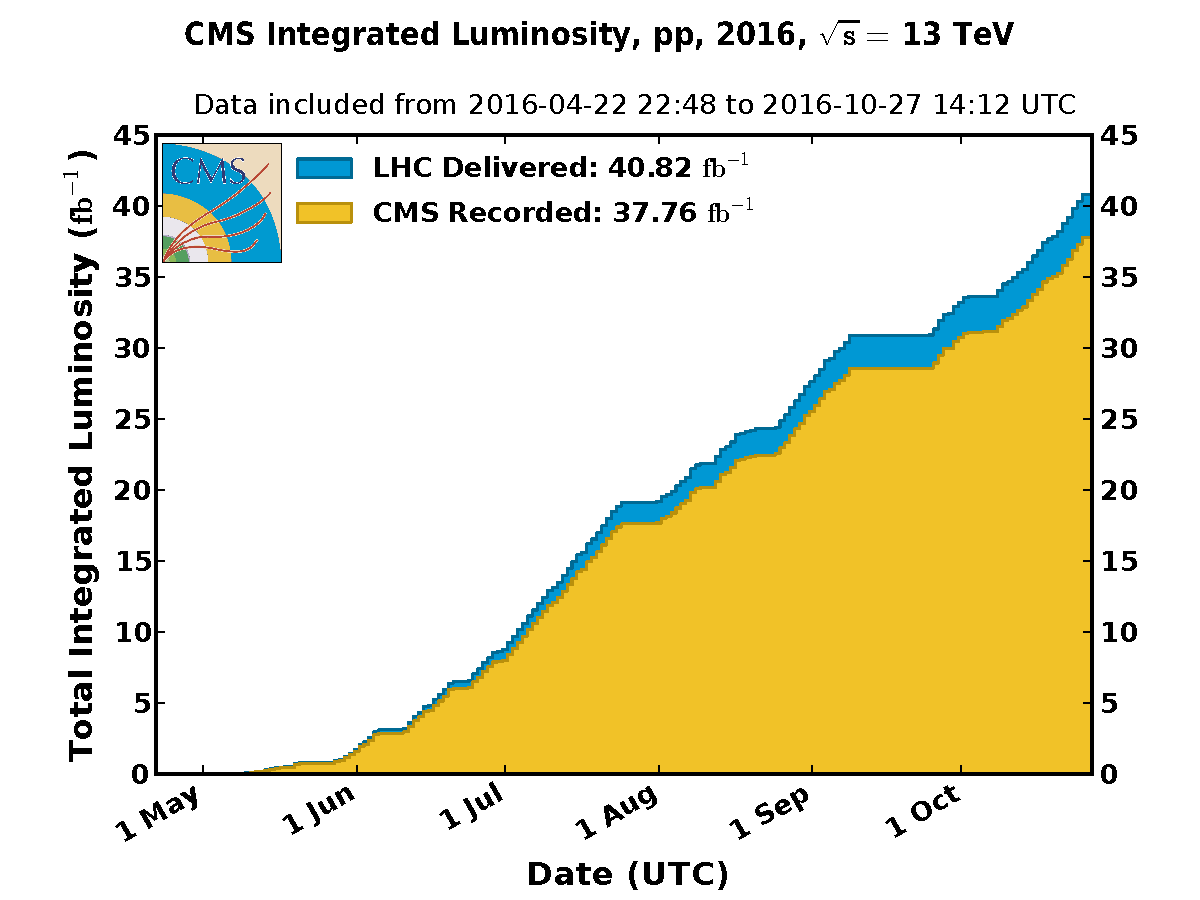
\includegraphics[width=0.7\textwidth]{2_ExperimentalSetup/Figures/int_lumi_per_day_cumulative_pp_2016.pdf}
	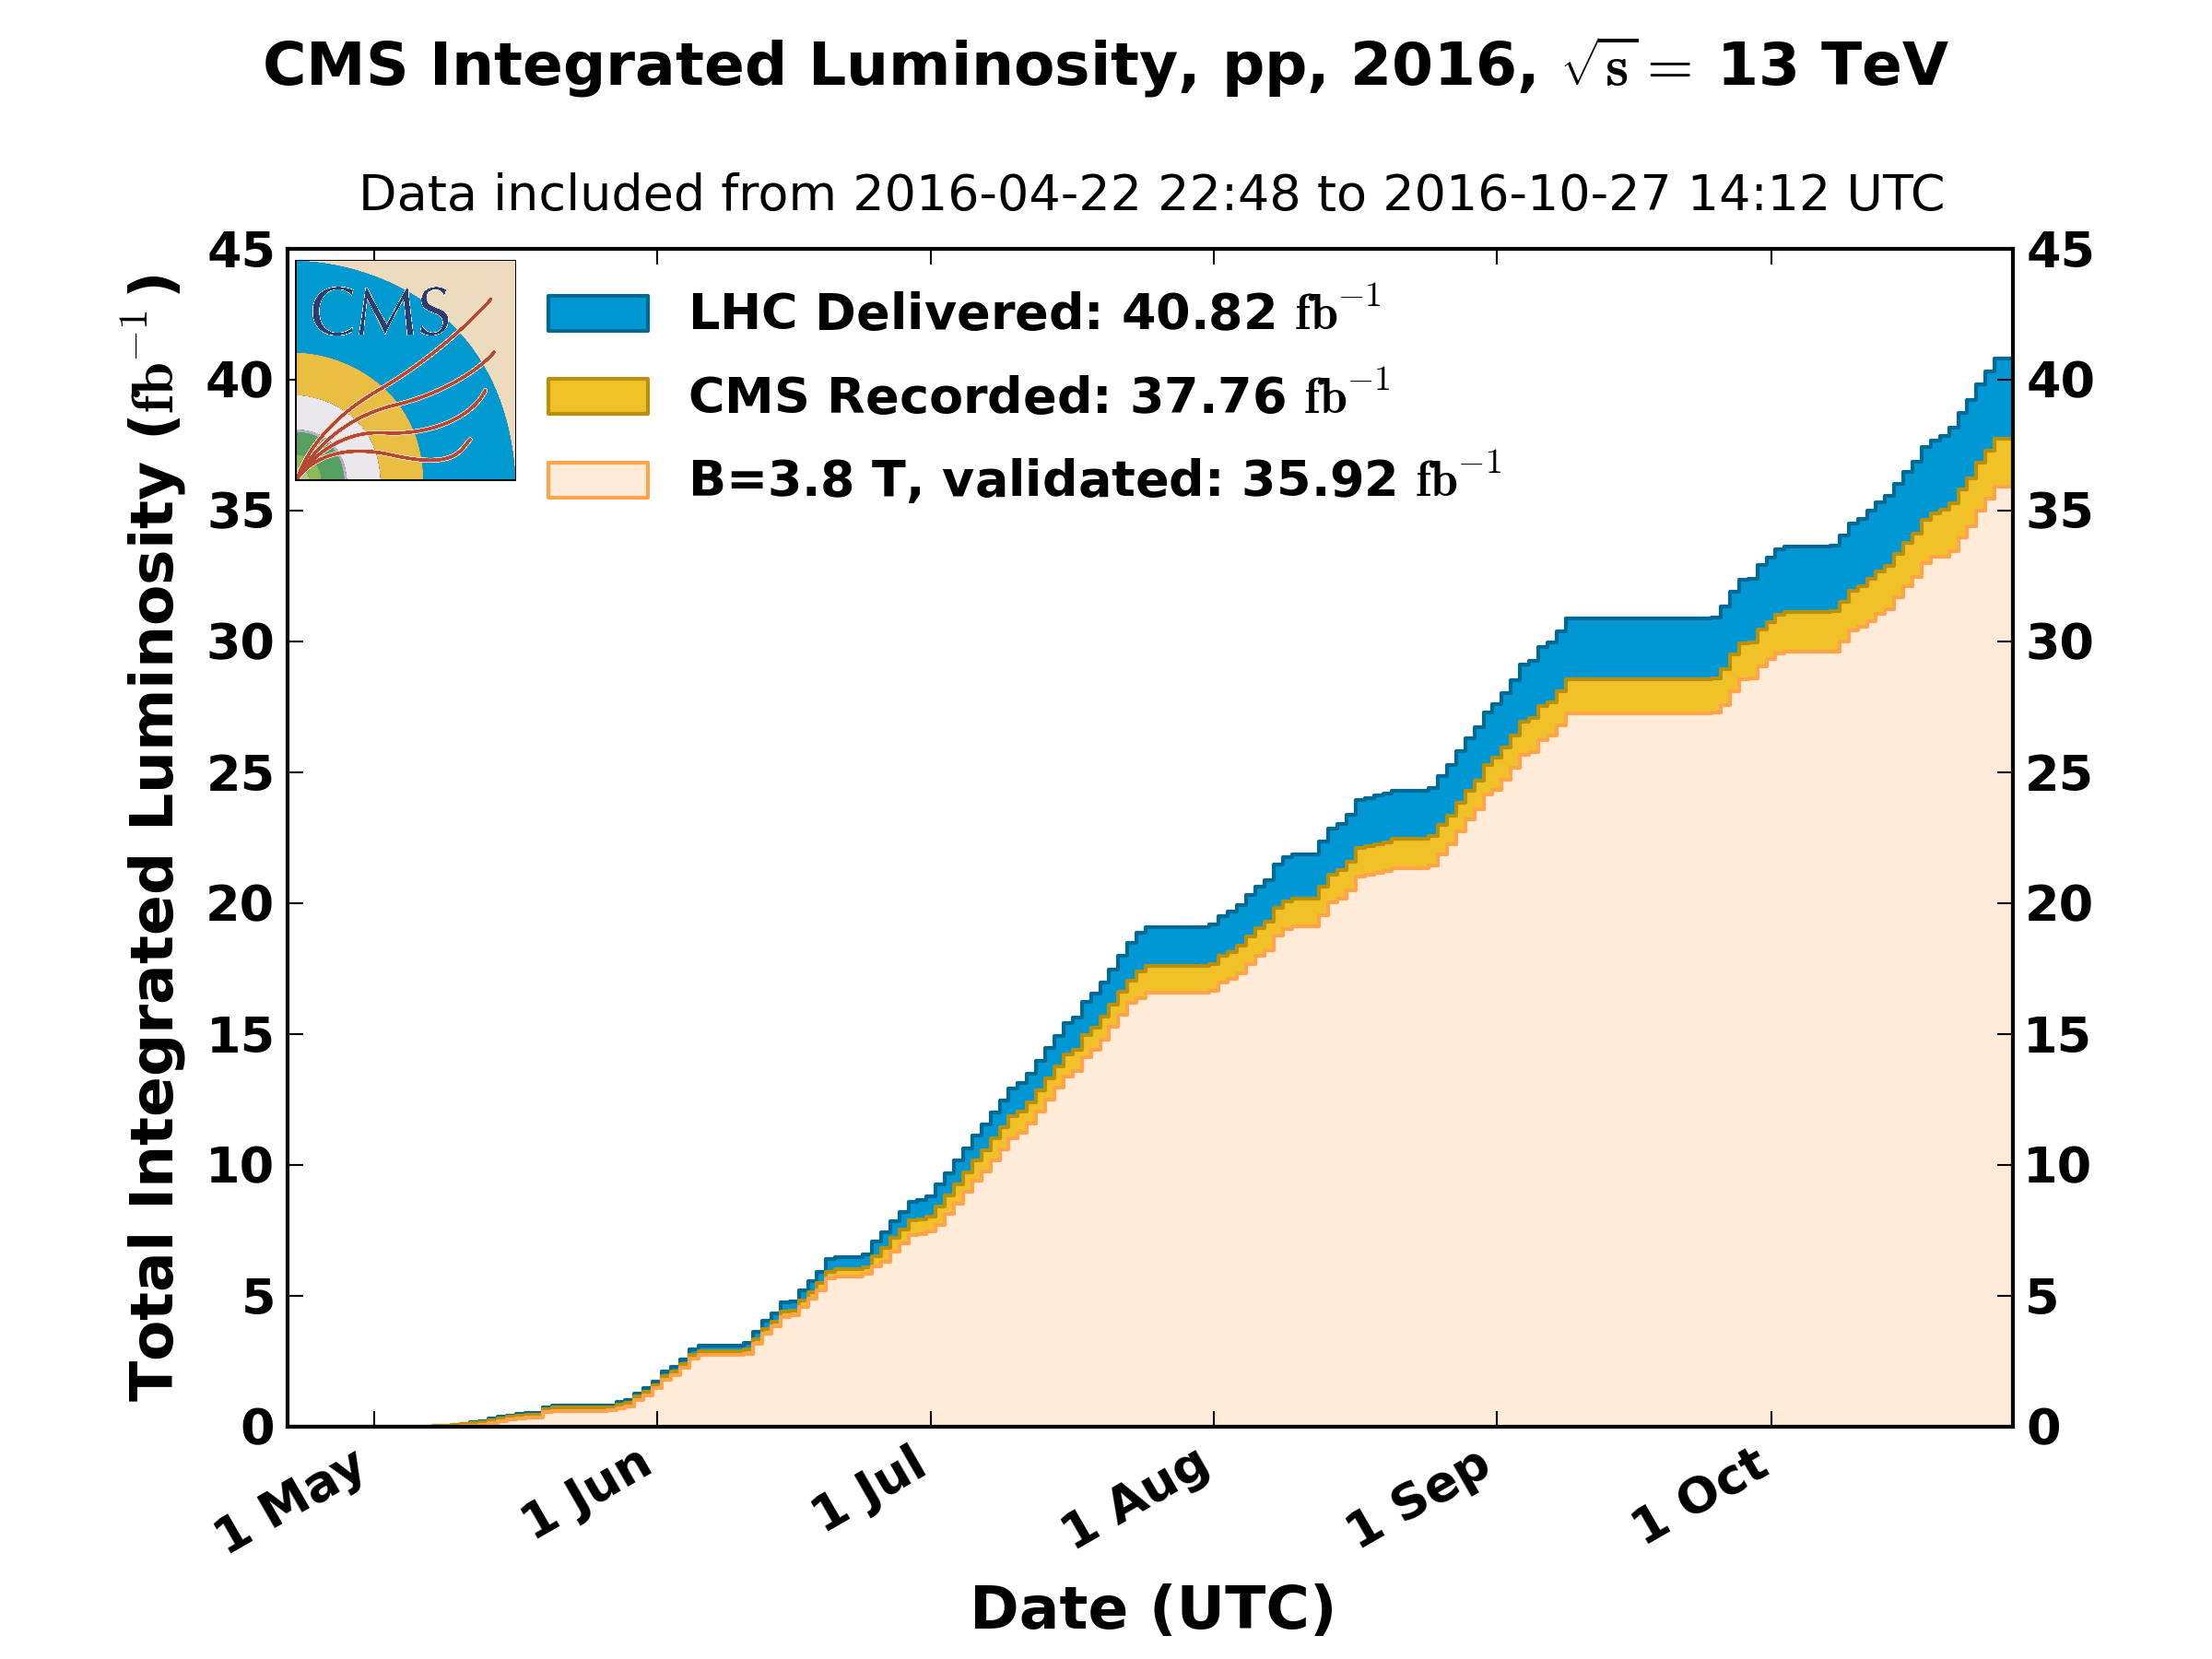
\includegraphics[width=0.7\textwidth]{2_ExperimentalSetup/Figures/int_lumi_per_day_cumulative_pp_2016_Golden_23Sep-PromEraH_Morion}
	\caption{Cumulative off-line luminosity measured versus day delivered by the LHC  (blue), and recorded by CMS (orange), and certified as good physics analysis during stable beams (light orange) during stable beams and for proton collisions at 13 TeV centre-of-mass energy in 2016.~\cite{LumiWiki}. }
	\label{fig:IntLumi}
%	(from https://twiki.cern.ch/twiki/bin/view/CMSPublic/LumiPublicResults#Online_Luminosity_AN2 )
%  https://twiki.cern.ch/twiki/bin/view/CMSPublic/DataQuality#2016_Proton_Proton_Collisions
\end{figure}
 
Multiple proton-proton interactions can occur during one  bunch crossing, referred to as \pu. On average, the number of \pu\ events is proportional to the luminosity times the total inelastic proton-proton cross section. In 2016,  an average of about 27 of \pu\ interactions has been observed in 13 \TeV\ proton collisions at the interaction point of CMS. For 2012, this number was about 21 \pu\ interactions for 8 \TeV\ collisions.



%CMS collaboration http://cds.cern.ch/record/2195940?ln=en map

% CMS Luminosity Measurement for the 2016 Data Taking Period`(CADI entry LUM-17-001)
% http://cms.cern.ch/iCMS/analysisadmin/cadi?ancode=LUM-17-001
\section{The Compact Muon Solenoid}
At one of the collision points of the LHC, the CMS detector\cite{CMS, Bayatian:2006zz,Bayatian:922757} is placed (see \fig{fig:CMS}). Weighing 14 000 \si{ \tonne}, This cylindrical detector is about 28.7 \si{ \meter} long and 15 \si{ \meter} in diameter, weighing around 14 000 \si{ \tonne}. It has an onion like structure of several specialised detectors and contains a superconducting solenoid with a magnetic field of 3.8 \si{ \Tesla}. The CMS detector is designed in a way that it can address the needs of physics coming from the LHC. Living in a hadronic environment, multi-jet processes produced by the strong interaction are a main source of background for rare physics processes. Therefore, good identification, momentum resolution, and charge determination of muon, electrons and photons is one of the main goals of the CMS detector. Further it provides a good charged particle momentum resolution and reconstruction efficiency in the inner tracker such that for example jets coming from b quarks or tau particles can be identified. Also the electromagnetic resolution for an efficient photon and lepton isolation as well as a good hadronic calorimeter for the missing transverse energy were kept into account while designing CMS. 

The LHC provides many collisions in a short amount of time. In order to discriminate between consecutive collisions - known as out of time pile up events - , CMS has to complete the full data acquisition for one collision event before the next one happen (around 25 \si{ \nano \second} in Run II and around 50 \si{ \nano \second} in Run I \cite{OLuanaigh:2051986}). Furthermore, since the photons are in packets, around 21 in Run I and 40 in Run II  inelastic collisions happen every beam crossing . This creates a great amount of background processes in the detector called in time pile up events. Due to this difficult conditions, the detector has a great granularity which on its turn creates a need for huge number of synchronized electronic channels. Furthermore, due to to high flux of particles in the regions close to the beam, the electronics has to be able to endure high radiation.


\begin{comment}
     \begin{figure}[ht]
	\centering
	\begin{minipage}[b]{0.4\textwidth}
		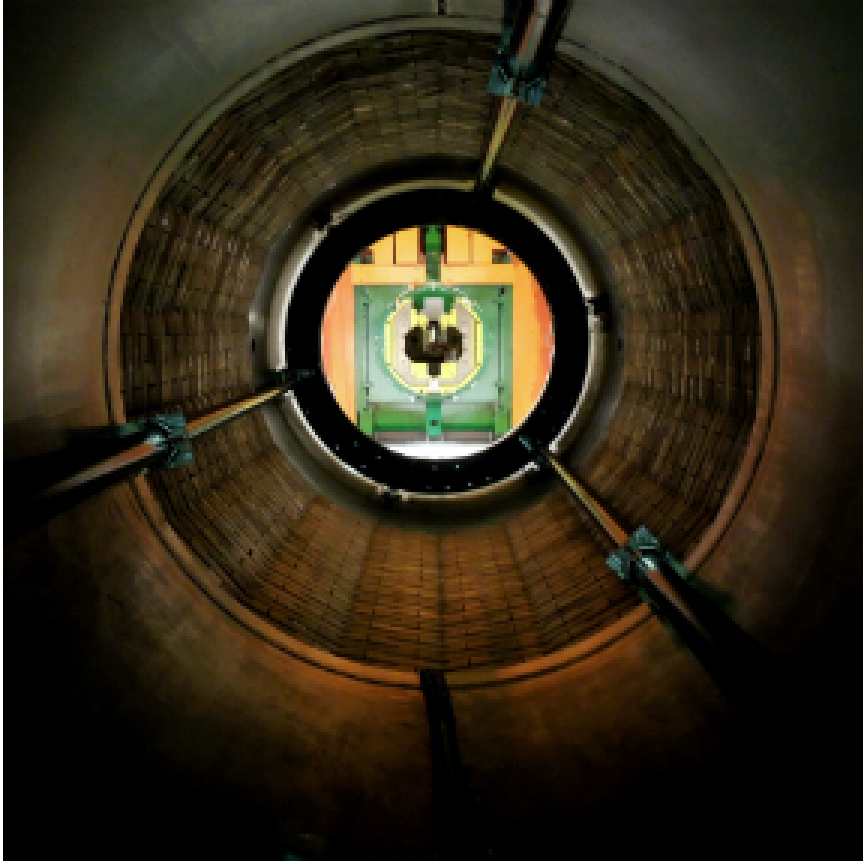
\includegraphics[width=\textwidth]{2_ExperimentalSetup/Figures/Beampipe}
		\caption{The LHC beampipe shown from inside CMS.(FIXME: use better resolution)}
	\end{minipage}
	\hfill
	\begin{minipage}[b]{0.4\textwidth}
		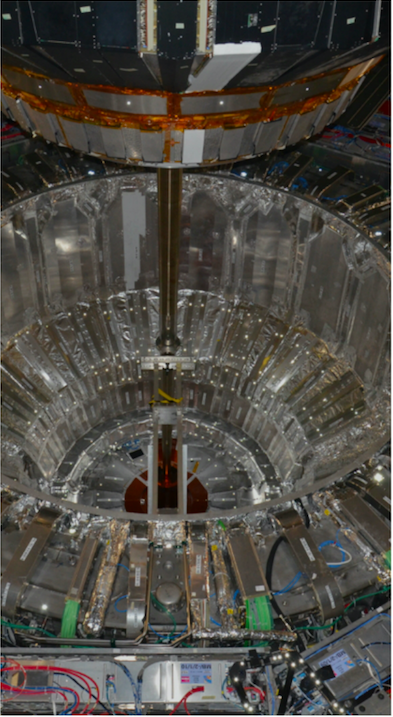
\includegraphics[width=\textwidth]{2_ExperimentalSetup/Figures/beampipe2}
		\caption{Beampipe going inside CMS. Picture taken from below (FIXME: use better resolution)}
	\end{minipage}
	\label{fig:IntLumi}
	%	(from https://twiki.cern.ch/twiki/bin/view/CMSPublic/LumiPublicResults#Online_Luminosity_AN2 )
\end{figure}
\end{comment}

\begin{figure}[ht]
	\centering
	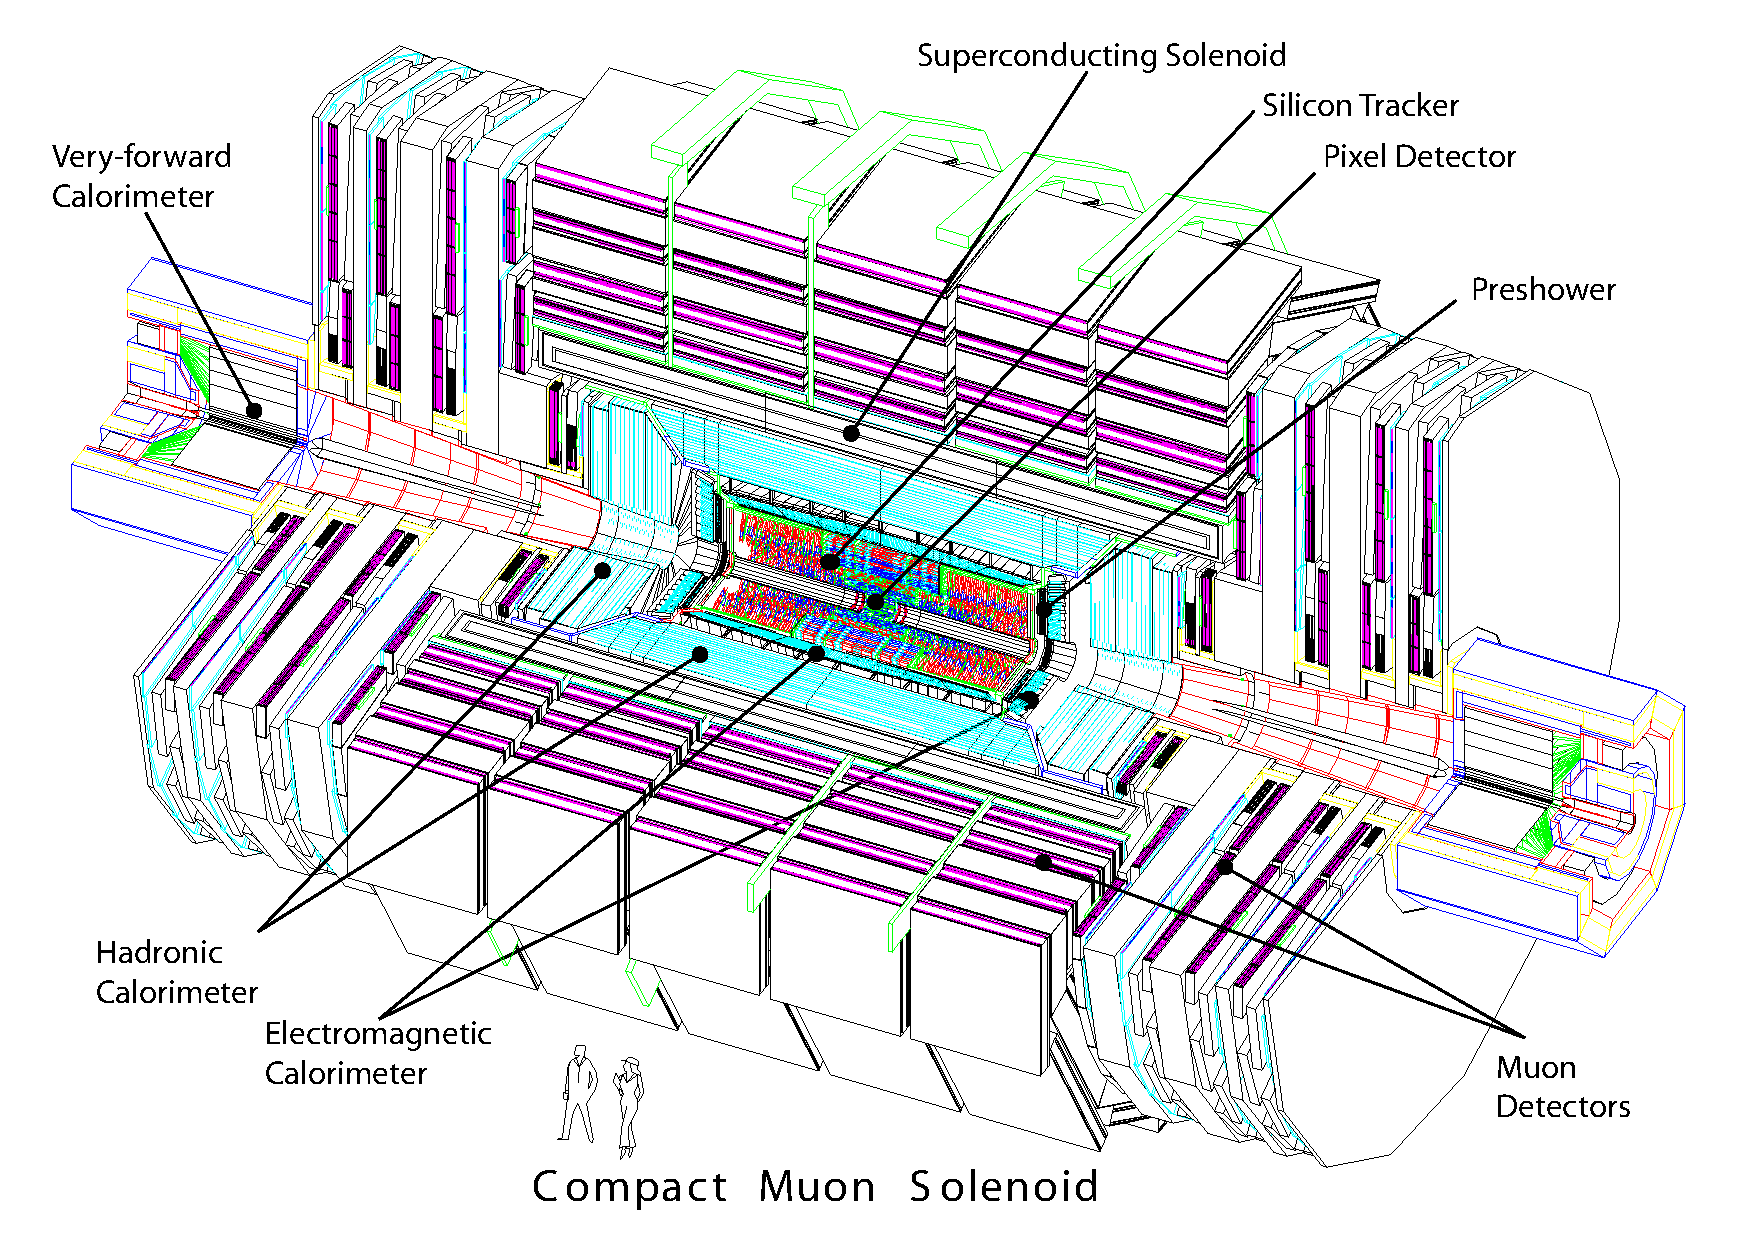
\includegraphics[width=\textwidth]{2_ExperimentalSetup/Figures/cms_complete_labelled}
	\caption{Mechanical layout of the CMS detector\cite{CMSdraw}.}
	\label{fig:CMS}
\end{figure}

Before the start of taking collision data for 13 \si{ \TeV} operations on 3 June, CMS had a long shutdown (LS1)\cite{Pralavorio:2024977}. During this shut down several upgrades were performed. The innermost part of detection material in CMS (pixel) is currently made of three concentric cylindrical layers. At the end of 2016 it is upgraded by adding a fourth layer, enhancing the particle tracking capabilities of CMS. In order to be able to incorporate this new layer, the section of the beryllium beam pipe within CMS was replaced by a narrower one during LS1. For this, the pixel was removed and reinserted into CMS.  In order to avoid long damage caused by the intense particle flux at the heart of CMS, the tracker is been made ready to operate at much lower temperature than before. During Run I, a small problem was detected in the electromagnetic calorimeter preshower system. For this, the preshower discs were removed, repaired and reinstalled successfully inside CMS in 2014. To help the discrimination between interesting low momentum muons coming from collisions and muons caused by backgrounds, a fourth triggering and measurement station for muons was added in each of the end caps.  CMS measures the collision rate within the detector and monitors beam related backgrounds. For this, several new detectors were installed into CMS during LS1. 


\newpage
\subsection{CMS coordinate system}
The coordinate system used by CMS can be found in \fig{fig:CMScoord}. The origin of the right handed orthogonal coordinate system is chosen to be the point of collisions. The x-axis points towards the centre of the LHC ring such that the y-axis points towards the sky, and the z-axis lies tangent to the beam axis. Since the experiment has a cylindrical shape, customary coordinates are used to describe the momentum \impuls: the distance $\rho$, the azimuthal angle $\phi \in \left[-\pi,\pi\right]$ - the angle between the x-axis and the projection in the transverse plane of \impuls (\trimpuls) - , the pseudo-rapidity \psrap - expressed by the polar angle $\theta$ between the direction of \impuls and the beam - : 
\begin{equation}
\eta = - \ln \left(\tan \left(\frac{\theta}{2}\right)\right).
\end{equation}
For the energies considered at the LHC, where $E >> m$, the pseudo-rapidity is a good approximation of the rapidity $y$
\begin{equation}
y = \frac{1}{2} \ln \left(\frac{E + p_z}{E - p_z}\right), 
\end{equation}
where the difference of rapidities of two particles is invariant under a Lorentz boost in the z-direction.
 \begin{figure}[ht]
	\centering
	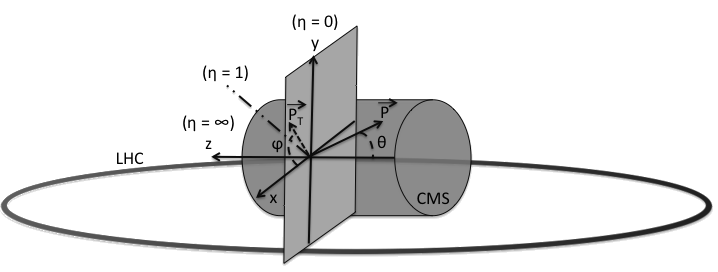
\includegraphics[width=0.75\textwidth]{2_ExperimentalSetup/Figures/imageedit_1_9146672677}
	\caption{Representation of the coordinate system used by CMS. The point of origin is put at the collision point. The x-axis points towards the centre of the LHC ring such that the z-axis lies tangent to the beam axis. }
	\label{fig:CMScoord}
\end{figure}

\subsection{Towards the heart of CMS}
The CMS detector consists of two parts; a central barrel around the beam pipe (\abspsrap $<1.4$) and two plugs to ensure the hermeticity of the detector. In \fig{fig:CMS} and \fig{CMSview} the onion like structure of the CMS detector is visible. The choice of a solenoid of 12.9 \si{ \meter}  long and 5.9 \si{ \meter}
diameter gives the advantage of bending the particle trajectories in the transverse plane. The hadronic calorimeter,  the electromagnetic calorimeter and the tracker are within the solenoid, while the muon chambers are placed outside the solenoid.



\begin{figure}[ht!]
	\centering
	\includegraphics[width=0.45\textwidth]{2_ExperimentalSetup/Figures/cmsview1}
	\includegraphics[width=0.45\textwidth]{2_ExperimentalSetup/Figures/cmsview}
 \caption{Schematic view of the CMS detector in the Run I configuration. (LEFT) Longitudinal view of one quarter of the detector. (RIGHT)  Transversal view of one quarter of the detector. The muon system barrel elements are denoted as MBZ/N/S, where z$=-2...+2$ is the barrel wheel number, n$=1...4$ the station number and S$=1...12$ the sector number. Similary, the steel return yokes are denoted as YBZ/N/S. The solenoid is denoted as CB0, while the hadronic calorimeter is denoted as HE (end cap)/ HB (barrel)/HF(forward) and the electromagnet calorimeter as EE(end cap)/EB (barrel). The green part represents the tracking system\cite{Chatrchyan:1223944}}.
	\label{fig:CMSview}
\end{figure}

\subsubsection{Muon system}
The outermost part of CMS consists of the muon system. The magnet return yoke is interleaved with gaseous detector chambers for muon identifictaion nd momentum measurement. The barrel contains muon stations arranged in five separate iron wheels, while in the end cap four muon stations are mounted onto three independent iron discs in on each side. Each barrel wheel as 12 sectors in the azimuthal angle. 

The muon system is divided into three parts\cite{Chatrchyan:1223944}, shown in \fig{fig:muonsys}. The muon rate and neutron induced backgrounds are small and the magnetic field is very low for the barrel and CMS can use drift tube (DT) chambers. For the end caps however, the muon and background flux is much higher and there is a need to use cathode strip chambers (CSC) which are able to provide a faster response, higher granularity and a better resistance against radiation. In order to form a redundant trigger system, resistive plate chambers (RPC) are added. This makes a total of 250 DT chambers, 540 CSC and 610 RPC. In \fig{fig:CMSview} the arrangement is shown.


\begin{figure}[ht!]
	\centering
	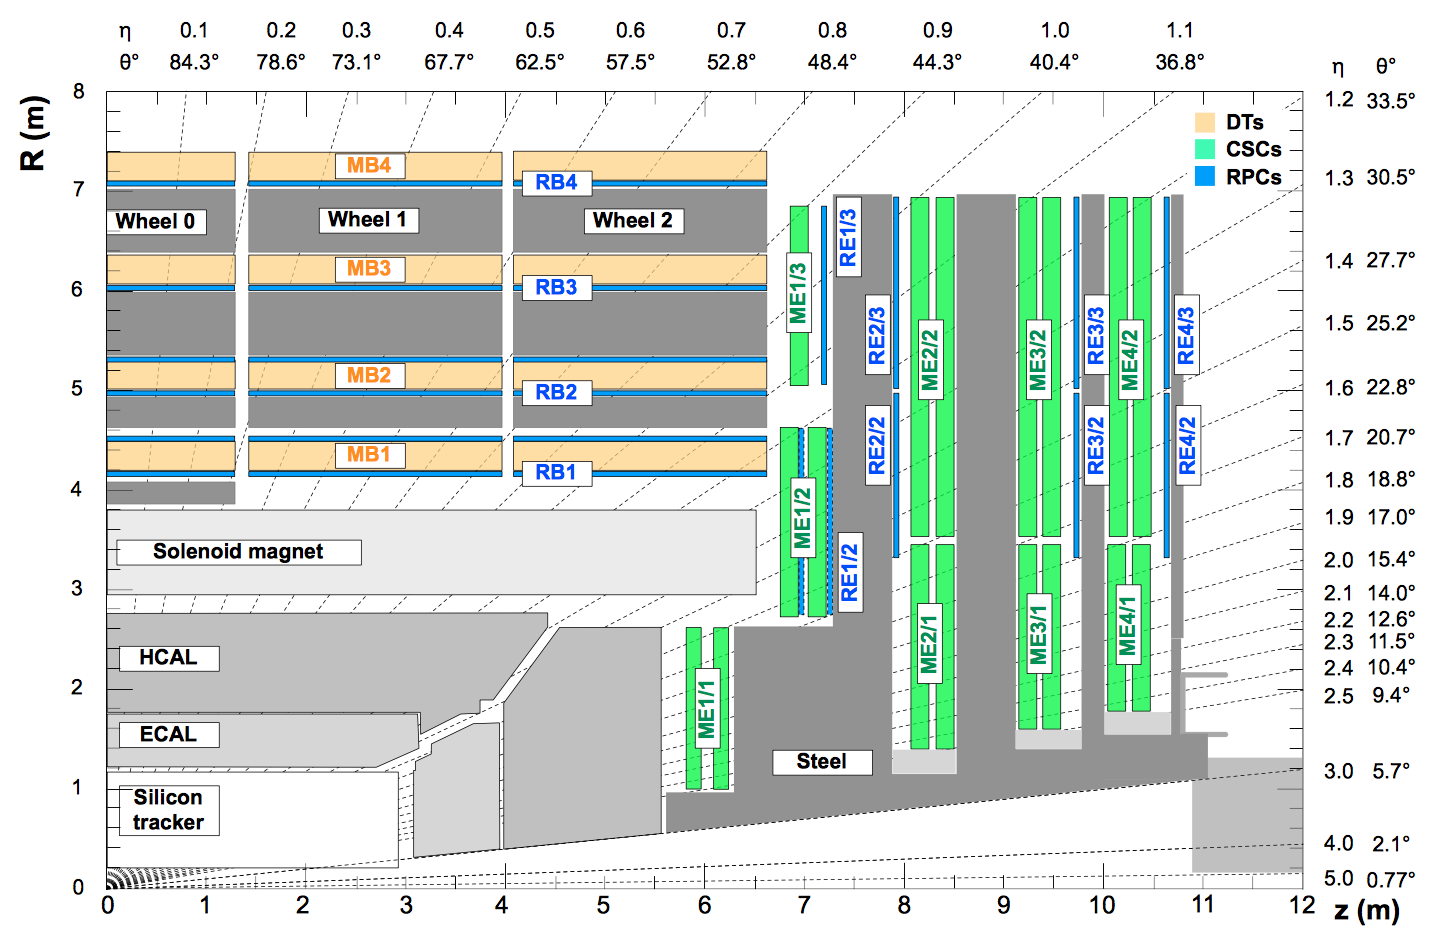
\includegraphics[width=0.6\textwidth]{2_ExperimentalSetup/Figures/muonsys}
	\caption{Schematic view of one quarter of the CMS muon system in the Run I configuration. \cite{Chatrchyan:1223944}}.
	\label{fig:muonsys}
\end{figure}


Providing a measurement for \abspsrap $<1.2$. The DT chambers in the barrel are on average 2 $\times$ 2.5 \si{ \meter} in size and consist of 12 layers of DT cells - 4 \si{ \centi \meter} wide gas tubes with positively charged stretched wire inside - arranged in three groups of four. The $r\phi$ coordinate is provided by the two outside groups, while the middle group measures the $z$ coordinate. For each $\phi$ sector, the DT chamber is mixed with the flux return yoke. For the outer muon station, the DT chamber contains only 8 layers of DT cells, providing a muon position in th $r\phi$ plane.
There are four CSC stations in each end cap, providing muon measurements for $0.9<$ \abspsrap $<2.4$ (Run I configuration). These CSC are multi-wired proportional chambers that consist of 6 anode wire planes crossed by 7 copper strips cathode panels in a gas volume. The $r$ coordinate is provided by the copper strips, while $\phi$ coordinate comes from the anode wires, giving a two dimensional position measurement. 
There are six layers of RPC in the barrel muon system and one layer into each of the first three stations of the end cap. They are made from two high resistive plastic plates with an applied voltage and separated by a gas volume. Read out strips mounted on top of on of the plastic plates detects the signal generated by a muon passing through the gas volume. The RPC provides a fast response with a time resolution of 1 \si{ \nano \second} and cover a range of \abspsrap $<1.8$ (Run I configuration). 


During the long shutdown, the  muon system underwent major upgrades~\cite{Guiducci:1966038,Battilana:2239185}. In the fourth station of each end cap, the outermost rings of CSC and RPC chambers were completed, providing an angular region of $1.2<$ \abspsrap $<1.8$ for Run II, increasing the system redundancy, and allowing tighter cuts on the trigger quality. In order te reduce the environmental noise, outer yoke discs have been placed on both sides for the end caps. 
At the innermost rings of the first station, the CSC has been upgraded by refurbishing the readout electronics to make use of the full detector granularity instead of groups of three (Run I). 


The muon system provides triggering on muons, identifying muons and improves the momentum measurement and charge determination of high $p_T$ muons. On top of the muon system, the muon energy is deposited in the electromagnetic calorimeter, the hadronic calorimeter, and outer calorimeter. (FIXME not tracker?) The high magnetic field enable an efficient first level trigger and allows a good momentum resolution of $\Delta ^p / p \approx 1\%$ for a $p_T$ of 100 \si{ \GeV} and $\approx 10\%$ for a $p_T$ of 1 \si{ \TeV} (FIXME). There is an efficient muon measurement up to \abspsrap $<2.4$.
\subsubsection*{Muon reconstruction}
% see http://www.bo.infn.it/sminiato/sm16/03_Mercoledi/Mattina/01_Battilana.pdf
% see https://arxiv.org/pdf/1510.05424.pdf
% see https://twiki.cern.ch/twiki/bin/view/CMSPublic/MuonDPGPublic160729
 The muon reconstruction\cite{Chatrchyan:2012xi} has three subdivision: local reconstruction, regional reconstruction and global reconstruction. 
The local reconstruction is performed on individual detector elements such as strip and pixel hits in the inner tracking system, and muon hits and/or segments on the muon chambers. Independent tracks are reconstructed in the inner tracker - called tracker track -  and in the muon system, called standalone tracks.
Based on these tracks, two reconstructions are considered.
The outside-in approach is referred to as Global Muon reconstruction. 
 For each standalone track, a tracker track is found by comparing the parameters of the two tracks propagated onto a common surface. Combining the hits from the tracker track and the standalone track, gives a fit via the Kalman filter technique~\cite{FRUHWIRTH1987444,Billoir:1989mh} for a global muon track. 
 The second approach is an inside-out reconstruction, creating tracker muons. 
 All candidate tracker tracks are extrapolated to the muon system taking into account the magnetic field, the average expected energy losses, and multiple Coulomb scattering in the detector material. When at least one muon segment - DT or CSC hits -  matches the extrapolated track, the corresponding tracker track is indicated as a tracker muon. 
 
 For low transverse momenta ($p_T \lesssim$ 5 \si{ \GeV}), the tracker muon reconstruction is  more efficient than the global muon approach. This is due to the fact that tracker muons only require a single muon  segment in muon system, while the global muon approach requires typically segments in at least two muon stations. Therefore, the global muon approach typically improves the tracker reconstruction for $p_T\gtrsim$ 200 \si{ \GeV}.
 The tming 

\subsubsection{Solenoid}
	Making use of the knowledge of previous experiments of ALEPH and DELPHI at LEP and H1 at HERA, CMS choose for a large super conducting solenoid with a a length of 12.9 \si{ \meter} and a inner bore of 5.9 \si{ \meter}\cite{Bayatian:922757}. With 2 168 turns, a -current of 19.5 \si{ \kilo \ampere} and  a total energy of 2.7 \si{ \giga \joule}, a large bending power can be obtained for a modestly-sized solenoid. In order to ensure a good momentum resolution in the forward regions, a favourable length/radius was necessary.  In \fig{fig:CMSsolenoid}, a photo of the CMS solenoid is given. 

	The solenoid uses a high-purity aluminium stabilised conductor with indirect cooling from liquid helium, together wit fully epoxy impregnation. A four-layer winding is implemented that can withstand an outward pressure of 64 \si{ \atm}. The NbTi cable is co-extruded by pure aluminium that acts as a thermal stabilizer and has an aluminium alloy for mechanical reinforcement. The return of the magnetic field is done by fives wheels, noted by YB in \fig{fig:CMSview}.
	
	\begin{figure}[ht]
		\centering
		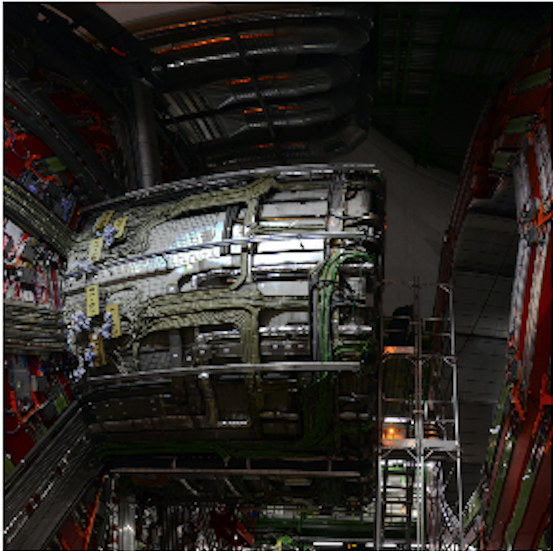
\includegraphics[width=0.45\textwidth]{2_ExperimentalSetup/Figures/solenoid}
		\caption{CMS solenoid during the long shutdown in 2013. }
		\label{fig:CMSsolenoid}
	\end{figure}	
	
\subsubsection{Hadronic calorimeter}
% http://cds.cern.ch/record/2235509?ln=en peformance
The hadronic calorimeter (HCAL) is dedicated to precisely measure the energy of charged and neutral hadrons via a succession of absorbers and scintillators. This makes it crucial for physics analyses with hadronic jets or missing transverse energy. The HCAL extends between 1.77 $<r<$ 2.95 \si{ \meter} where $r$ is the radius in the transverse plane with respect to the beam. Due to space limitations, the HCAL needs to be as small as possible and is made from materials with short interaction lengths - the length needed for absorbing 36.7\% of the hadrons. The quality of the energy measurements is dependant on the fraction of the hadronic shower that can be detected. Therefore, the HCAL barrel (HB) inside the solenoid is reinforced by an outer hadronic calorimeter between the solenoid and muon detectors (HO, see \fig{fig:HCAL}), using the solenoid as extra absorber. This increases the thickness to 12 interaction lengths. Furthermore, it should be as hermetic as possible and extend to large pseudo rapidity values. The HB and HO provide measurements for \abspsrap $<1.3$, while an end cap on each side (HE,$1.3<$ \abspsrap $<3$) and a forward calorimeter (HF, \abspsrap < 5.2) extend the pseudo rapidity range. 


\begin{figure}[ht]
	\centering
	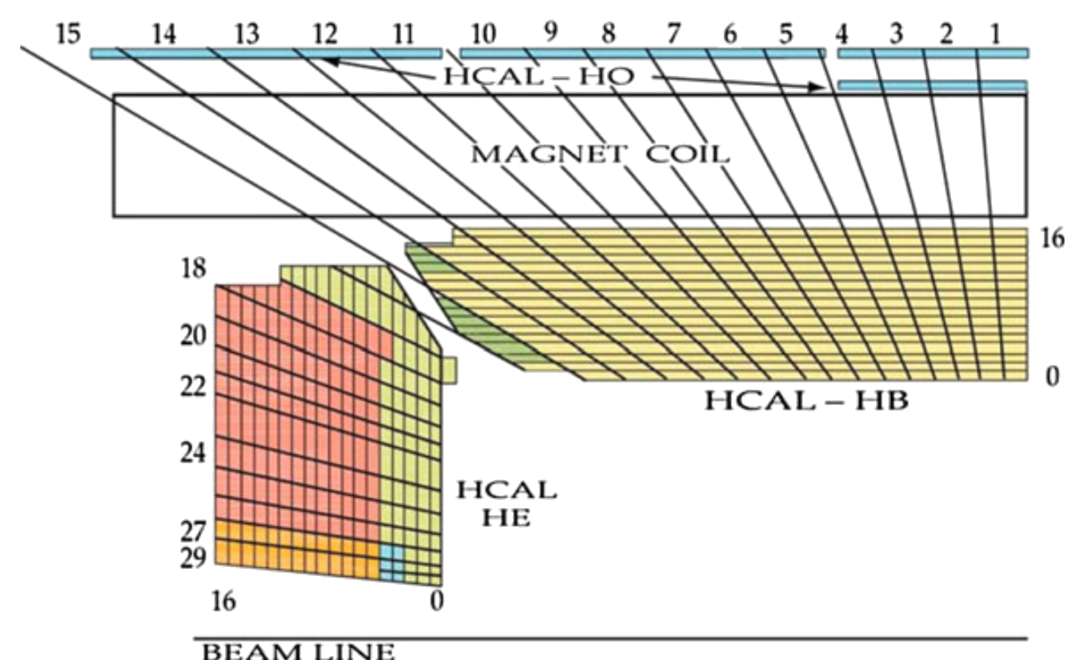
\includegraphics[width=0.5\textwidth]{2_ExperimentalSetup/Figures/imageedit_12_3242046754}
	\caption{Tower segmentation for one quarter of the HCAL displayed in the $rz$ plane\cite{Chatrchyan:2008aa}.}
	\label{fig:HCAL}
\end{figure}

The HB is made of 16 absorber plates where most of them are built from brass and others are made from stainless steal and is about five to ten intercation lengths thick. The HE is also composed of brass absorber plates and has a thickness corresponding to approximately ten interaction lengths. 
The HF experiences intense particle fluxes with an energy of 760 \si{ \GeV} deposited on average in a proton interaction at a center of mass of 14 \si{ \TeV}, compared to 100 \si{ \GeV} in the rest of the detector. Therefore, these are Cherenkov light detectors made of radiation hard quartz fibers.
The main causes of such large energy events is high energy muons, cosmic particles and charged particles from late showering hadrons. During  Run I, it became clear that the glass windows of the PMTs had to be replaced which was done during the long shut down \cite{Tiras:2016ghv}
	
\subsubsection{Electromagnetic calorimeter}
The electromagnetic calorimeter (ECAL) is designed to measure the energy of photons and electrons and covers \abspsrap $<3$. It is an hermetic, homogeneous detector and consists of 75 848 lead tungstate (PbW$O_4$) crystals. These crystals have a fast response time - 80\% of the light is emitted within 25 \si{ \nano \second} - and are radiation hard. The electromagnetic showers produced by passing electrons or photons ionize the crystal atoms which emit a blue-green scintillation light, that is collected by silicon avalanche photodiodes (APDs) in the barrel and vacuum phototriodes (VPTs) in the end caps. The crystals and the APD response is sensitive to temperature changes and require a stable temperature. 

\begin{figure}[ht]
	\centering
	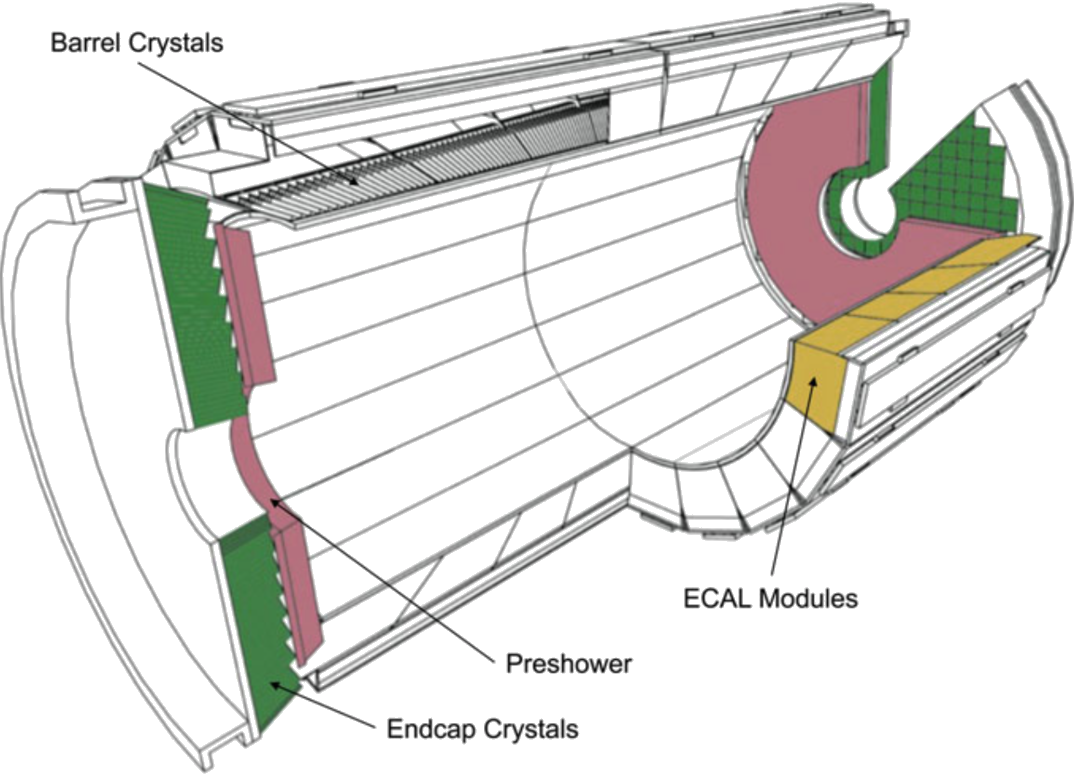
\includegraphics[width=0.5\textwidth]{2_ExperimentalSetup/Figures/imageedit_5_8264930617}
	\caption{Schematic cross section of the electromagnetic calorimeter\cite{Chatrchyan:2008aa}.}
	\label{fig:ECAL}
\end{figure}
There are three regions: a central barrel (EB), a endcap region (EE) and a preshower (ES) (\fig{fig:ECAL}). 
The EB has an inner radius of 129 \si{ \centi \meter} and corresponds to a pseudo rapidity of $0 < $ \abspsrap $<1.479$. At a distance of 314 \si{ \cent \meter} from the vertex and covering a pseudo rapidity of $1.479 < $ \abspsrap $<3.0$, are the EE. They consist of semi-circular aluminium plates from which structural units of $5\times5$ crystals (super crystals) are supported. The ES is placed in front of the crystal calorimeter over the end cap pseudo rapidity range with two planes of silicon strip detectors as active elements. 

The electromagnetic shower will typically involve more then one channel. More than 90\% of the energy of a 35 \si{ \GeV} electron or photon is contained in a $5\times 5$ matrix of crystals. Therefore, a clustering algorithm is performed in order to associate the energy deposits to the particles impinging the calorimeter.
The achieved precision\cite{1748-0221-12-01-C01069} for the barrel is 2.10$^{-3}$ \si{ \rad} in $\phi$ and 10$^{-3}$ in \psrap. For the end caps this is 5.10$^{-3}$ \si{ \rad} in $\phi$ and 2.10$^{-3}$ in \psrap. The energy is reconstructed by a super cluster algorithm, taking into account energy radiated via bremsstrahlung or conversion: 
\begin{equation}
E_{e/\gamma} = G F_{e/\gamma} \sum_{i \in cluster} S_i(t) VC_i A_i,
\end{equation}
where $G$ is the absolute energy scale in \si{ \GeV \per \ADC}, $F$ the energy containment corrections (depends on type of particle, its energy and pseudo rapidity, eg shower leakage and bremsstrahlung losses for electrons), $S(t)$ the relative channel variation with time, $C$ the relative channel response and $A$ the amplitude in \si{ \ADC} counts. The energy resolution is given by 
\begin{equation}
\frac{\sigma(E)}{E} = \frac{2.8\%}{\sqrt{E}}\oplus \frac{0.128}{E(GeV)} \oplus 0.3\%, 
\end{equation}
in the absence of a magnetic field, where the contributions come from the stochastic, noise and constant terms respectively. The dominating term is the constant term ($E_{shower} \approx 100 GeV$) and thus the performance is highly dependent on the quality of calibration and monitoring .

In Run I, the energy reconstruction happened  via a weighted sum of the digitized samples\cite{Chatrchyan:2013dga}. For Run II however, the reconstruction had to be made more resistant for out of time pile up and a multi-fit approach has been set in to place. In this approach, the pulse shape is modelled as a sum of one in-time pulse plus the out of time pulses \cite{1748-0221-12-01-C01069}. The energy resolution is less than 2\%  in the central barrel region and 2-5 \% elsewhere.
% https://indico.cern.ch/event/477407/contributions/2305075/attachments/1368970/2075215/hc16-edm.pdf
% see http://iopscience.iop.org/article/10.1088/1748-0221/12/01/C01069/pdf at vub
% http://www.bo.infn.it/sminiato/sm16/03_Mercoledi/Sera/08_Brianza.pdf
% https://indico.cern.ch/event/472938/contributions/1150724/attachments/1273518/1888397/ECALEnergyOverview_CALOR.pdf
%https://inspirehep.net/record/1344855/files/10.1088_1742-6596_587_1_012001.pdf
\begin{comment}
The relative energy resolution of the ECAL for electrons is between 1.4-3\% in EB and 3-4\% for EE. In Figure \ref{fig:ECALres}, the resolutions for low and high bremsstrahlung electrons are shown. 
\begin{figure}[ht]
	\centering
	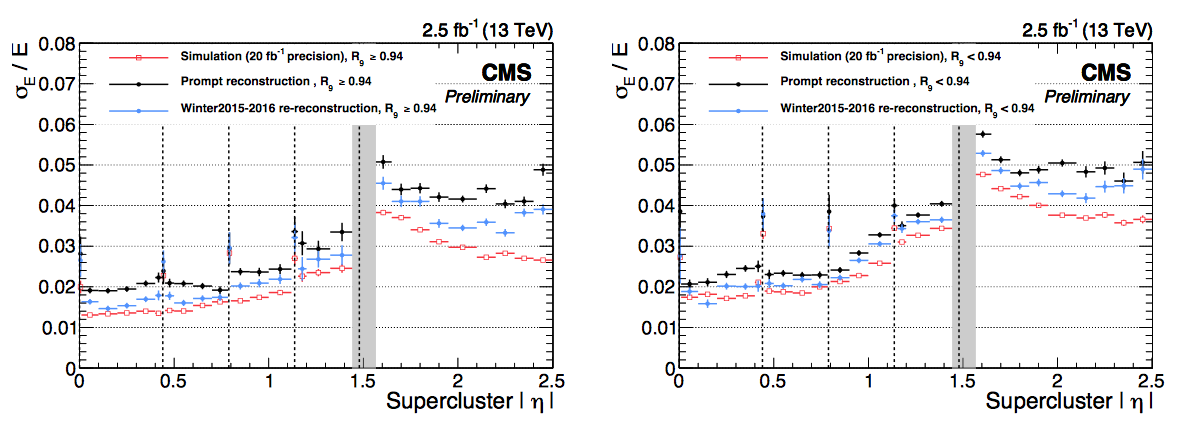
\includegraphics[width=\textwidth]{2_ExperimentalSetup/Figures/imageedit_7_5931623976}
	\caption{Relative energy resolution in bins of pseudo rapidity for the barrel and end caps using electrons from $Z \rightarrow ee$. Left: low bremsstrahlung electrons, Right: high bremsstrahlung electrons\cite{Sun:2233637}.}
	\label{fig:ECALres}
\end{figure}
\end{comment}

\subsubsection{Inner tracking system and operations}
%https://indico.cern.ch/event/632928/
%http://cds.cern.ch/search?ln=en&cc=CMS+Reports&sc=1&p=tracker&f=title&action_search=Search
% comparison with atlas https://cds.cern.ch/record/1563583/files/ATL-PHYS-PROC-2013-206.pdf
The tracking system (tracker)~\cite{Chatrchyan:1704291} is the detecting unit closest to the point of interaction. Responsible for the reconstruction of  trajectories from charged particles with \abspsrap $<2.5$, being bend by the magnetic field, it provides a measurement of the momentum. The tracker is also responsible for the determination of the interaction point or vertex. It should be able to provide high granularity as well as speed, and be able to endure high radiation. For this reason, the CMS collaboration choose silicon detector technology.

\begin{figure}[ht]
	\centering
%	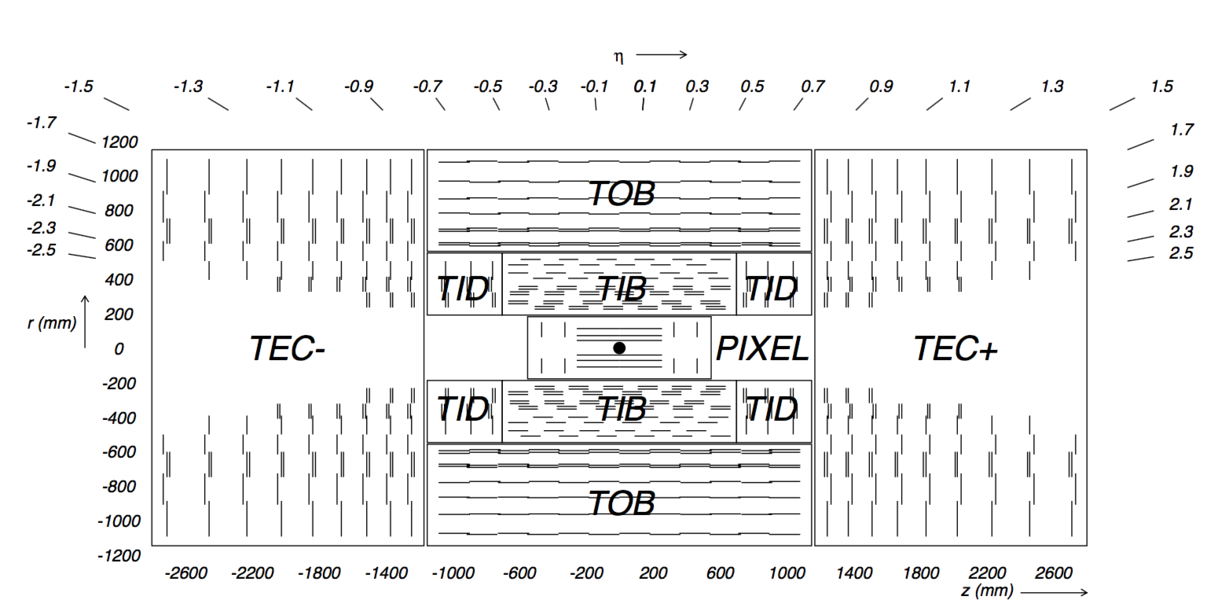
\includegraphics[width=\textwidth]{2_ExperimentalSetup/Figures/imageedit_3_5170744545}
	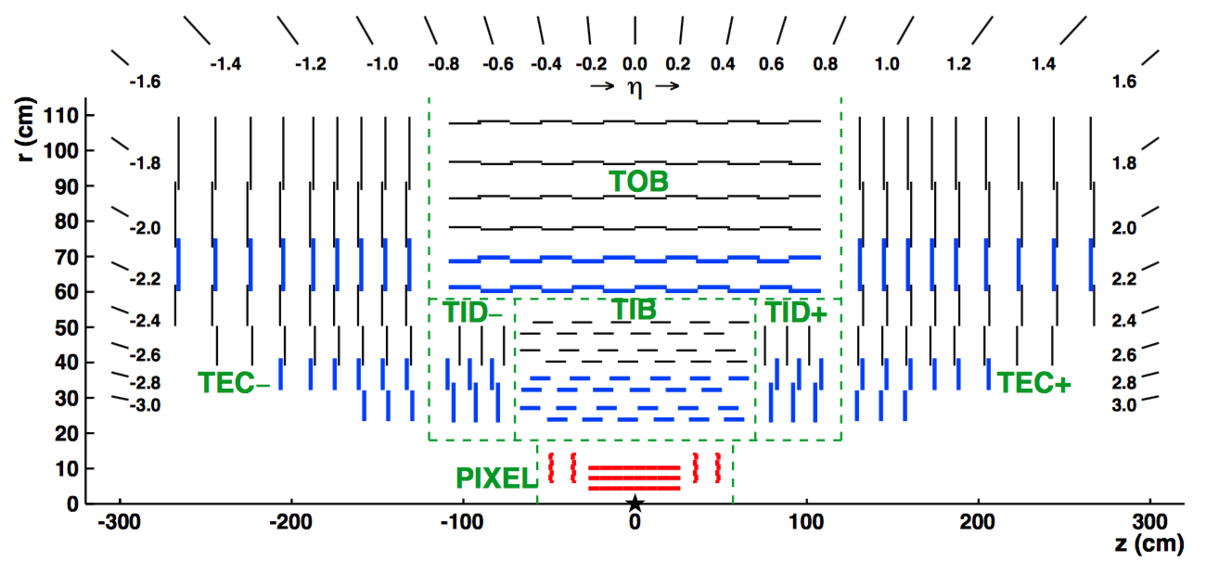
\includegraphics[width=0.7\textwidth]{2_ExperimentalSetup/Figures/imageedit_11_9317262269}
%	\caption{Schematic cross section through the CMS tracker. Each line represents a detector module. Double lines indicate back-to-back modules\cite{Chatrchyan:2008aa}.}
  \caption{Schematic cross section of the top half of the CMS tracking system in the $rz$ plane. The centre of tracker is shown with a star and corresponds to the approximate position of the proton collision point. The green dashed lines are an indication for each named tracker subsystem. The strip tracker modules that provide two-dimensional hits are shown by thin, black lines, while those able to reconstruct three-dimensional hit positions are shown by thick, blue lines. The pixel modules, shown in red, also provide three-dimensional hits. \cite{Bayatian:2006zz} }
	\label{fig:Tracker}
\end{figure}

 The tracking system consists of a cylinder of 5.8 \si{ \meter} long and 2.5 \si{ \meter} in diameter. It is immersed in a co-axial magnetic field of 3.8 \si{ \Tesla} due to the solenoid.
 As shown \fig{fig:Tracker}, the tracker is built up from a large silicon strip tracker with a small silicon pixel inside. 
 The inner region, pixel ($4.4<r<10.2$ \si{ \cm}), gets the highest flux of particles. Therefore, pixel silicon sensors of $100 \times 150$ \si{ \squared \micro \meter} is used. It consists of three cylindrical barrels that are complemented by two discs of pixel modules at each side.
 The silicon strip tracker ($20<r<116$ \si{ \cm} ) has three subdivisions. The Tracker Inner Barrel  and Discs (TIB, TID) are composed of four barrel layers accompanied by three discs at each end. The outer part of the tracker - Tracker Outer Barrel (TOB) -  consists  of 6 barrel layers. In the outer discs, there are nine discs of silicon sensors, referred to as Tracker End Caps (TEC). 
  
 
 The pixel, shown in \fig{fig:pix} has 1440 modules that cover an area of about 1 \si{ \squared \meter} and have 66 million pixels. It provides a three-dimensional position measurement of the hits arising from the interaction from charged particles with the sensors. In transverse coordinate ($r\phi$), the hit position resolution is about 10 \si{ \micro \meter}, while 20-40 \si{ \micro \meter} is obtained in the longitudinal coordinate ($z$). The sensor plane position provides the third coordinate. 
  The silicon strip trackers consists of 15 148 single sided modules placed in the TIB, TID and the first four rings of the TEC. They provide 9.3 million readout channels. In the TOB and the outer three rings of the TEC, double sided modules are used. These modules are constructed from two back-to-back single sided modules, where one module is rotated through a stereo angle.  This covers an active area of about 198 \si{ \squared  \meter}. The TIB and TID provide position measurements in $r\phi$ with a resolution of approximately 13-38 \si{ \micro \meter}, while the TOB provides a resolution of about 18-47 \si{ \micro \meter}. The resolution in the  $z$ direction is approximately 230  \si{ \micro \meter} in the TIB/TID and 530  \si{ \micro \meter} in the TOB. To allow overlay and avoid gaps in acceptance, each module is shifted slightly in $r$ or $z$ with respect to its neighbouring modules within a layer.  With this detector lay out, at least nine points per charged particle trajectory can be measured in an \abspsrap range up to 2.4.
  
  
       \begin{figure}[ht]
  	\centering
  	\begin{minipage}[b]{0.4\textwidth}
  		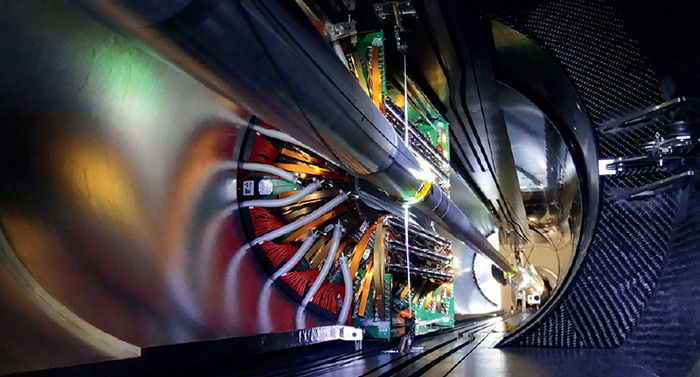
\includegraphics[width=\textwidth]{2_ExperimentalSetup/Figures/cmspixel}
  		\caption{The pixel barrel being re-installed after the Long Shutdown in 2015, around the beam pipe at CMS\cite{Christine:2024986}}
  		\label{fig:pix}
  	\end{minipage}
  	\hfill
  	\begin{minipage}[b]{0.4\textwidth}
  		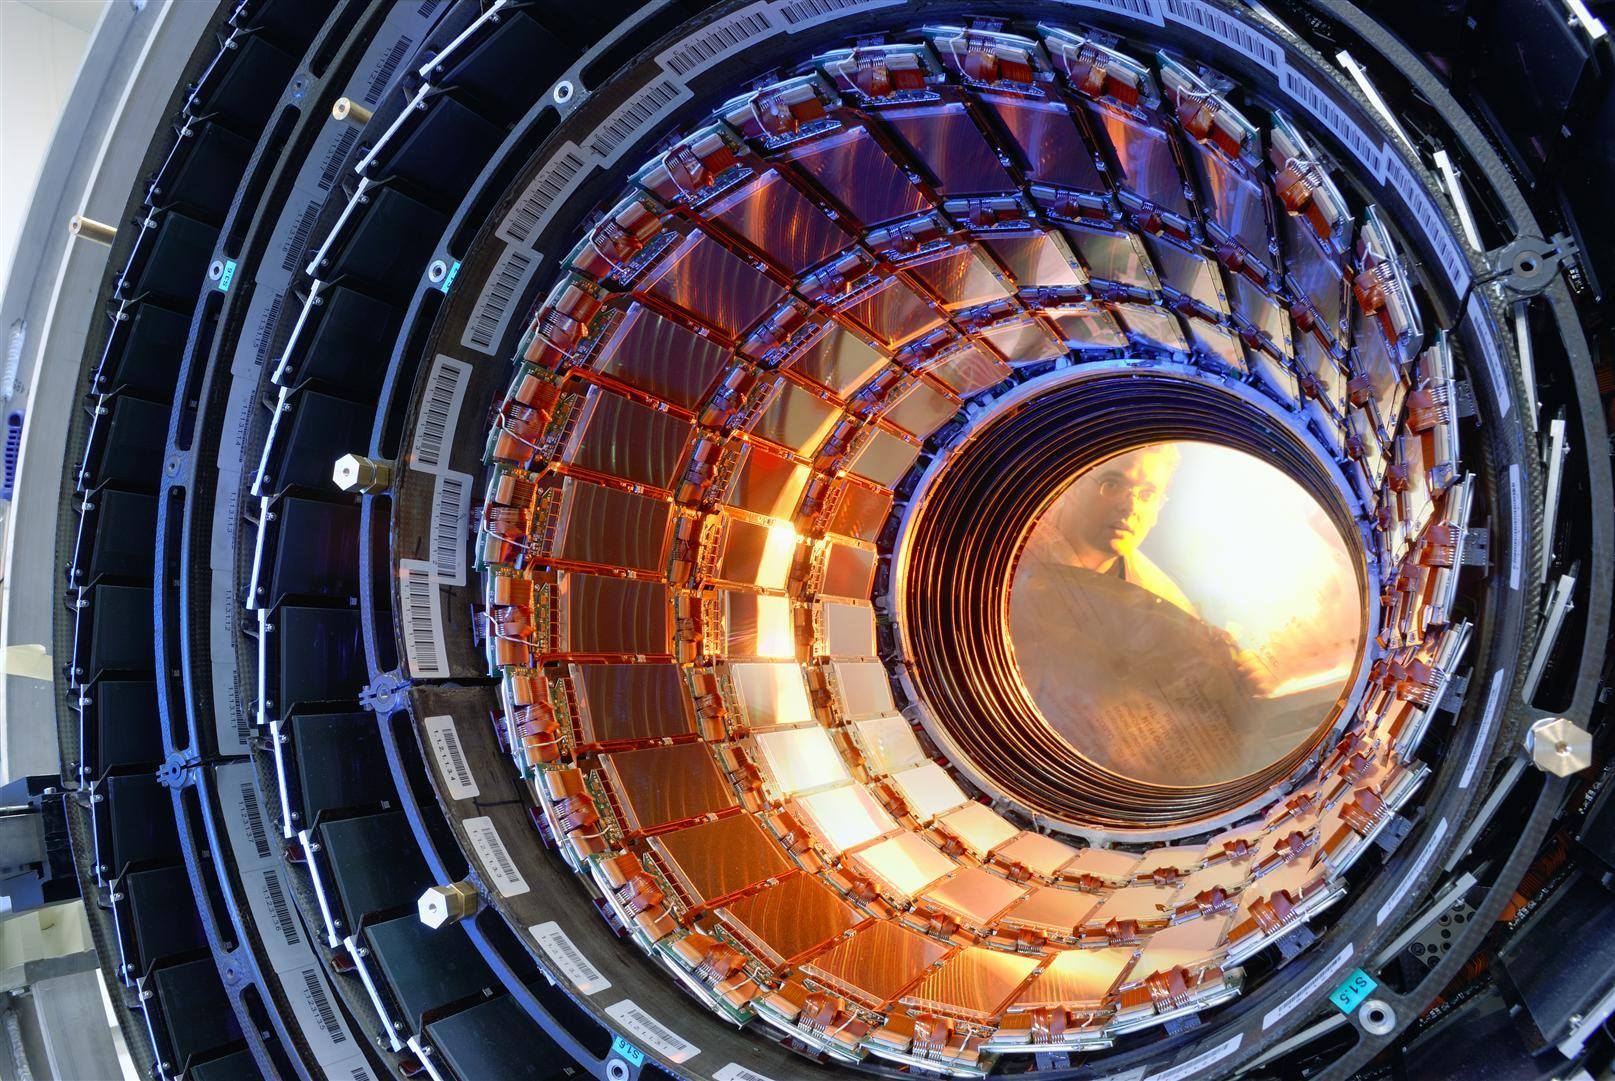
\includegraphics[width=\textwidth]{2_ExperimentalSetup/Figures/cmsbarrel}
  		\caption{First half of the inner tracker barrel, consisting of three layers of silicon modules.\cite{beautiful:1998635}}
  			\label{fig:Trackpics}
  	\end{minipage}
  
  	%	(from https://twiki.cern.ch/twiki/bin/view/CMSPublic/LumiPublicResults#Online_Luminosity_AN2 )
  \end{figure}
  
  
  
  
   During the first data taking period of the LHC (2010 to 2013), the tracker operated at +4\si{ \degree C}. With the higher LHC beam intensities from 2015 onwards, the tracker needs to be operated at much lower temperatures. This is due to the fact with intense irradiation, the doping concentration changes, the leakage current increases proportional to the fluence and the charge collection efficiency decreases due to charge trapping. Mostly the leakage current (I) is affected by the temperature change: 
   \begin{equation}
   I \propto T^2 e^{-\frac{E_g}{2kT}}, 
   \end{equation}
    where $T$ is the operating temperature, $E_g$ the band gap and $k$ the Boltzmann constant. There is approximately a factor 15 between the leakage currents at room temperatures and at $-10$ \si{ \degree C}. 
    % see http://www.hephy.at/user/friedl/diss/html/node14.html
    
    During the first long shutdown (LS1), the CMS cooling plant was refurbished\cite{running:1998606} and the fluorocarbon cooling system overhauled. To help to suppress the humidity inside the tracker, new methods for vapour sealing and insulation were applied. Furthermore, several hundred high-precision sensors are used to monitor the humidity and temperature. In order to get as dry air as possible, a new dry-gas plant provides eight times more dry gas (air or nitrogen) than during the first run, and allows regulation if the flow. As final addition, the cooling bundles outside the tracker are equipped with heater wires and temperature sensors in order to maintain safe operations above the cavern dew point For the data taking in 2015-2016, the tracker operated at $-15$\si{ \degree C}.
    
     \begin{figure}[ht]
    	\centering
    	\begin{minipage}[b]{0.3\textwidth}
    	%	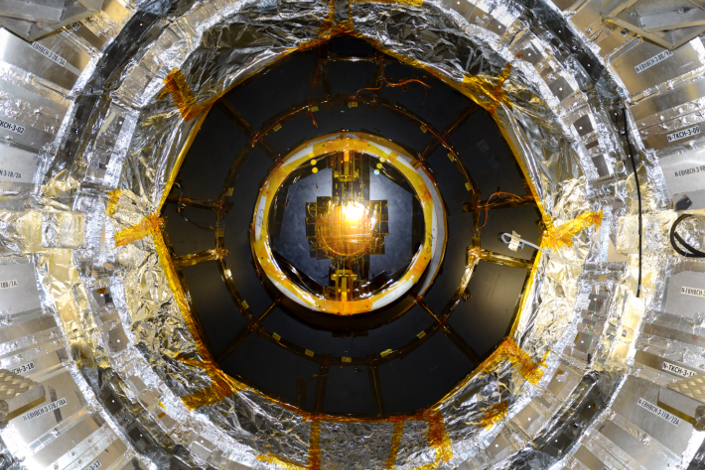
\includegraphics[width=\textwidth]{2_ExperimentalSetup/Figures/Tracker_bulkhead}
    	\includegraphics[width=\textwidth]{2_ExperimentalSetup/Figures/BHIsis}
    		\caption{Tracker bulkhead being put into closed state with insulation pieces installed during an early trial in fall 2013}
    	\end{minipage}
    	\hfill
    	\begin{minipage}[b]{0.5\textwidth}
    	%		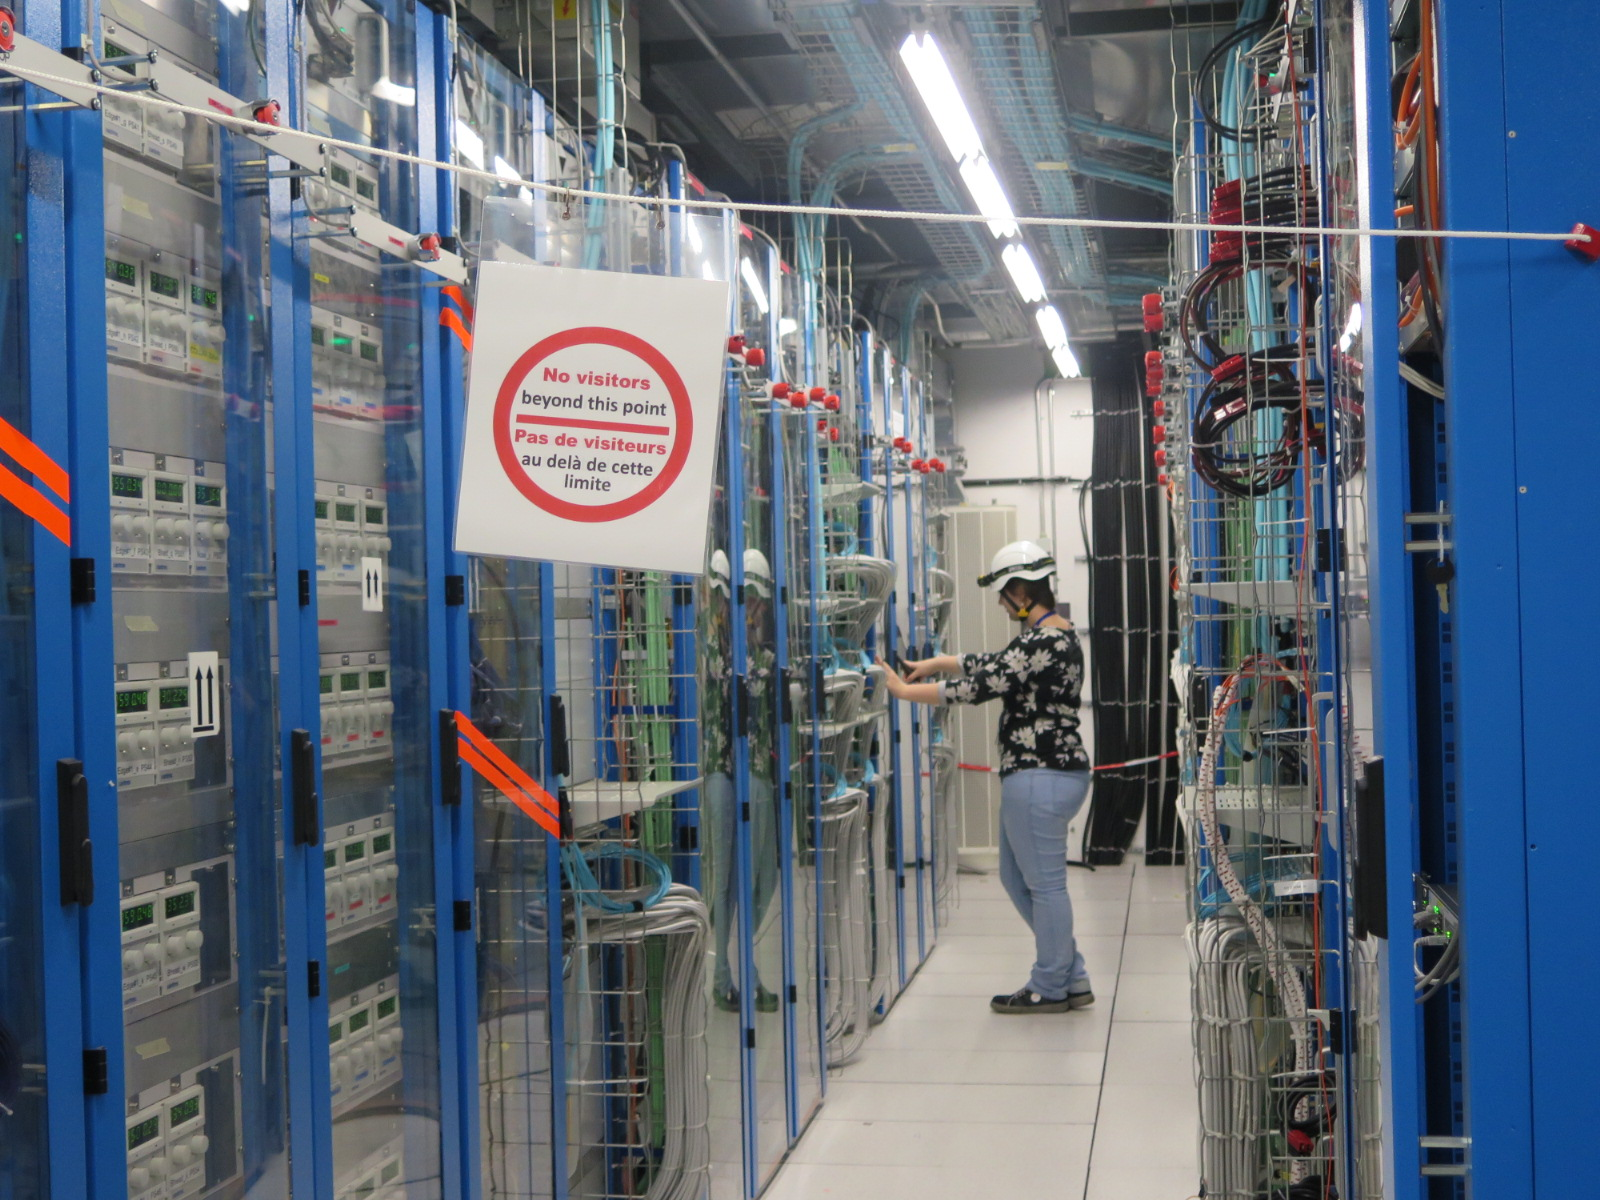
\includegraphics[width=\textwidth]{2_ExperimentalSetup/Figures/IMG_0138}
    	%	\caption{Tracker service racks containing the electronics coming from the tracking systems.}
    	
    		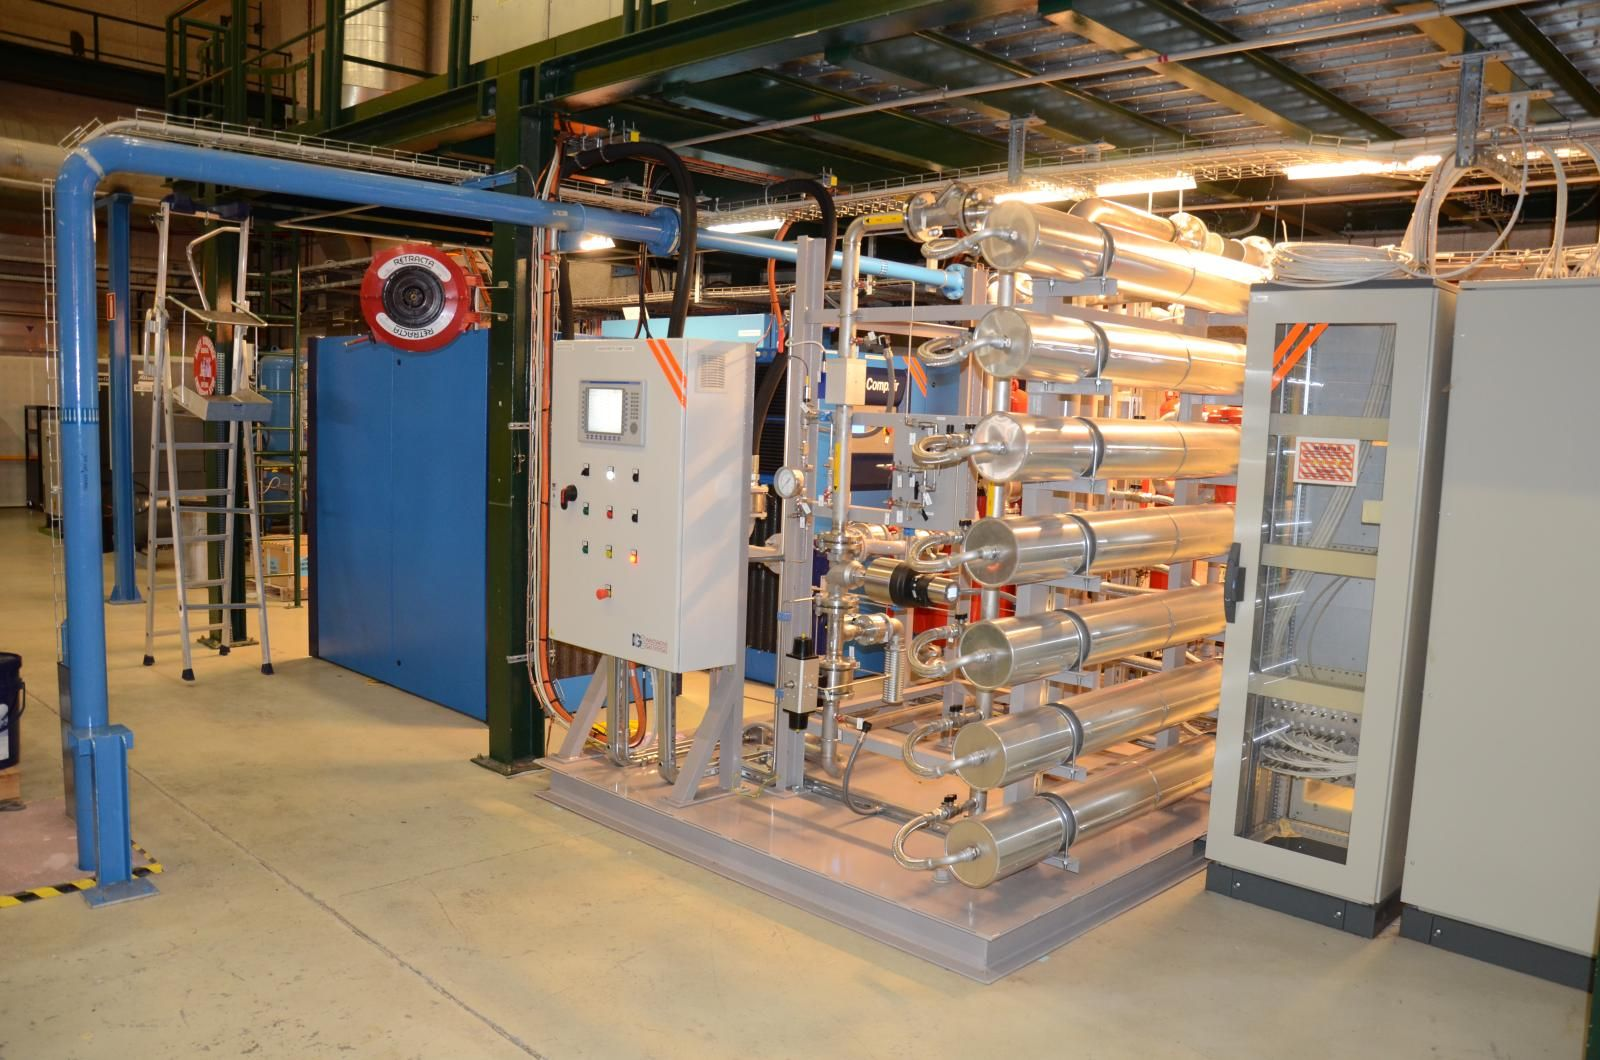
\includegraphics[width=\textwidth]{2_ExperimentalSetup/Figures/plant}
    		\caption{New Tracker high-capacity dry-gas plant with membrane separation system\cite{Pralavorio:2024977}}
    	\end{minipage}
    	\label{fig:TrackLS1}
    	%	(from https://twiki.cern.ch/twiki/bin/view/CMSPublic/LumiPublicResults#Online_Luminosity_AN2 )
    \end{figure}

\subsubsection*{Track reconstruction}
% see also https://arxiv.org/pdf/physics/0512097.pdf
% https://cds.cern.ch/record/1563583/files/ATL-PHYS-PROC-2013-206.pdf
% http://cds.cern.ch/record/1704291
An iterative tracking algorithm is responsible for the reconstruction of the tracks made by charged particles in the inner tracking system. Each iteration consists of four steps\cite{Bayatian:922757}: the track-seed generation, the pattern recognition algorithm, removal of track-hit ambiguities and a final track fit. 

The seed generation is the first step. It consists of finding reconstructed hits that are usable for seeding the subsequent track-finding algorithm. They are identified from a group of at least three reconstructed hits in the tracker, or from a pair of hits while requiring the origin of the track segment to be compatible with the nominal beam-collision point. Since the pixel has a higher granularity compared to the strip tracker, its seed generation efficiency is higher. The overall efficiency exceeds 99\%.
The second step of each iteration, the pattern recognition algorithm, uses the seeds as a starting point for a Kalman filter method~\cite{FRUHWIRTH1987444,Billoir:1989mh}. This algorithm extrapolates the seed trajectory towards the next tracker layer taking into account the magnetic field and multiple scattering effects. The track parameters are updated when a compatible hit in the next layer is found. This procedure continues until the outermost layer us reached.
Since the Kalman filter method can result in multiple tracks associated to the same seed, or different tracks sharing the same hits, a removal of ambiguities is necessary. This ambiguity resolving is done by removing tracks that are sharing too many hits from the list of track candidates. The tracks with highest number of hits or with the lowest $\chi^2$ if the track fit is kept. 
The updated track parameters are then refitted using the Kalman filter method, where all hits found in the pattern recognition step are taken into account. The fit is done twice - once outwards from the beam line towards the calorimeters, and inwards from the outermost track hit to the beam line -, improving the estimation of the track parameters. 

All hits that are unambiguously associated to the final track are removed from the list of available hits. In order to associate the remaining hits, the procedure is repeated with looser track reconstruction criteria. The use of the iterative track reconstruction procedure has a high track finding efficiency, where the fake track reconstruction rate is negligible. 
For muons, this results in a global track reconstruction efficiency exceeding 98\%, and 75-98\% for charged hadrons. Due to the lack of coverage of the two pixel discs in high \abspsrap range, the efficiency drops. 
%The resolution on the transverse momentum for a 100 \si{ \GeV} charged particle is about 2.0\% (FIX ME). 
% see https://twiki.cern.ch/twiki/bin/view/CMSPublic/TrackingPOGPlots2016
\subsubsection*{Primary vertex reconstruction}
The primary vertex reconstruction should be able to meausre the location of all proton interaction vertices in each event: the signal vertex an all vertices from pile up events. 
It consists of a vertex finding and a vertex fitting algorithm and happens in three steps. Tracks are selected  to be consistent with being produced promptly in the primary interaction by imposing requirements on track parameters\cite{Chatrchyan:1704291} By grouping reconstructed tracks according to the $z$ coordinate of their closest approach to the beam line, vertices for all interaction in the same beam crossing are found, at CMS this is done by a deterministic annealing algorithm~\cite{726788} . On top of this, a vertex fitting algorithm like the Adaptive Vertex fitter~\cite{Waltenberger:1166320}, is performed. This creates the three-dimensional primary-vertex position. With this fit, the contribution from long-lived hadron decays is reduced by down weighting the tracks with a larger distance to the vertex. The primary vertex corresponding to the highest sum of squared track transverse momenta is noted as the point of the main interaction. The resolution on the primary vertex is about 14 \si{ \micro \meter} in $r\phi$ and about 19 \si{ \micro \meter}) in the $z$ direction for primary vertices with the sum of the track $p_T > 100$ \si{ \GeV} for 2016 data taking.
% numbers from https://twiki.cern.ch/twiki/bin/view/CMSPublic/TrackingPOGPlotsICHEP2016
\subsection{Data acquisition}
% event display https://cds.cern.ch/record/2242076/files/DP2017_001.pdf
At a design luminosity of 10$^{34}$ \si{ \per \square \meter \per \second}, the proton interaction rate exceeds 1 \si{ \giga \hertz}. This makes it impossible for the CMS experiment to store all the data generated. For this, a two level trigger system has been put in place. The first level (Level-1) is a custom hardware system, while a second level (HLT) is software based running on a large farm of computers. 
In run II, with the increase in centre of mass energy and a higher luminosity a larger number of simultaneous inelastic collisions per crossing is expected with respect to run I. For this, the CMS Level-1 has been upgraded~\cite{1748-0221-12-03-C03021}. 

\subsubsection*{CMS Level-1 trigger}
The Level-1 trigger has to be a flexible, maintainable system, capable of adapting to the evolving physics programme of CMS~\cite{Khachatryan:2016bia}. Its output rate is restricted to 100 \si{ \kilo \hertz} imposed by the CMS readout electronics. It is implemented by custom hardware and selects events containing candidate objects - eg ionization deposits consistent with a muon, or energy clusters corresponding to an electron / photon / tau lepton / missing transverse energy / jet. Collisions with large momenta can be selected by using scalar sum of the transverse momenta of the jets. 

\begin{comment}
\begin{figure}[h]
	\centering
	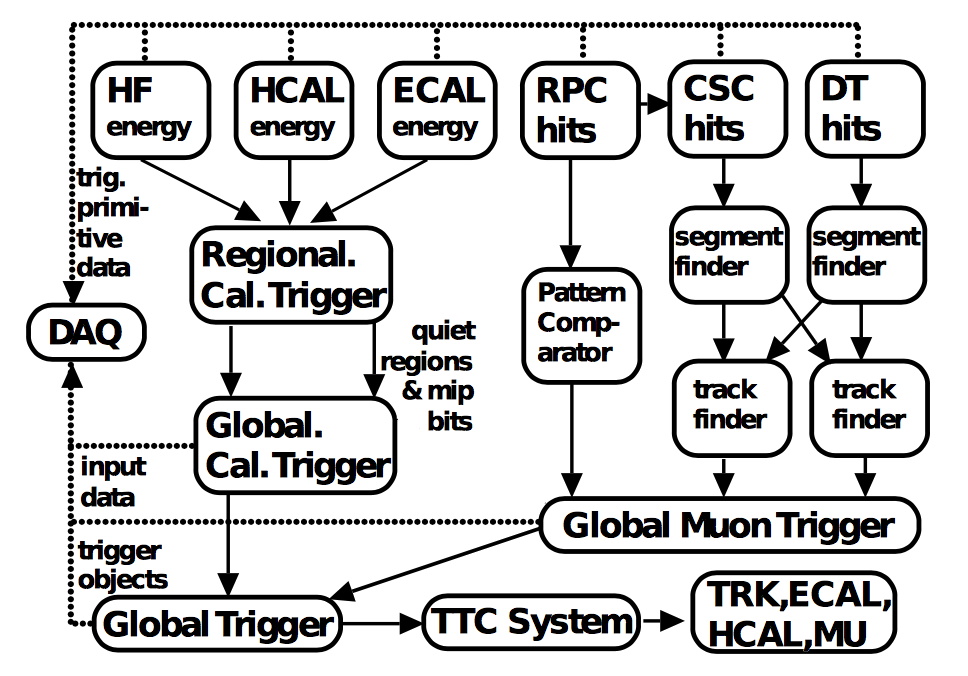
\includegraphics[width=0.5\linewidth]{2_ExperimentalSetup/Figures/imageedit_13_6388071145}
	\caption{The CMS level 1 trigger system for run I. Data from the calorimeters are processed regionally (RCT) ad the globally (GCT). Data from the muon chambers are processed via a global muon trigger (GMT). A global trigger (GT) combines the GCT and GMT, making a trigger decision. Th data acquisition system (DAQ) reads data from the tracker (TRK) via the trigger, timing  and control (TTC) system \cite{Khachatryan:2016bia}.}
	\label{fig:level1}
\end{figure}
\end{comment}

By buffering the raw data from the CMS subdetectors in front-end drivers, the level-1 trigger has a pipeline memory of 3.2 \si{ \micro \second} to decide whether to keep an event or reject it. 
%In \fig{fig:level1} the structure of the trigger is shown. 
The trigger primitives (TP) from the calorimeters and muon detectors are processed in several steps and combined into a global trigger. This information is then combined with the input from the other subsystems. The seperate inouts are synchronized to each other and the LHC orbit clock and sent to th eglobal trigger module. Here, level-1 trigger algorithms are performed within 1 \si{ \micro \second} to decide whether to  keep the event. 

For run II, all hardware, software, databases and the timing control system have been replaced. The main changes are that the muon system now uses the redundancy of three muon detector system earlier to make a high resolution muon trigger. The calorimeter system isn't bound any more for streaming data the data and the global trigger has more level-1 trigger algorithms. 
% see https://indico.cern.ch/event/432527/contributions/1072399/attachments/1320545/1980311/ichep2016.pdf

\subsubsection*{CMS HLT trigger}
The HLT is an array of commercially available computers with programmable menu that has output rate of on average 400 \si{ \hertz} for off-line event storage.
The data processing is based on a HLT path. This is a  set of algorithmic steps to reconstruct objects and make selections on them.  Here, the information of all sub detectors can be used to perform algorithms on higher level reconstructed objects. 
(FIXME: tracker in hlt or already in L1? )
\subsection{CMS computing model}
The selected data is stored, processed and dispersed via the Worldwide Large Hadron Collider GRID (WLCG)\cite{Grandi:814248,Eck:840543}. This has a tiered structure that function as a single, coherent system:. 

At CERN, a single Tier-0 is located. The raw data collected by CMS is archived here, and a first reconstruction of the data is done. This data is then in a file format usable for physics analysis. Furthermore, it is able to reprocess data when new calibrations are made available. The Tier-0 site distributes this data to a total of seven Tier-1 centres. They carry out data reprocessing and store real data as well as simulated  data. The Tier-1 further distribute the data to over 50 Tier-2 centres. These make the data accessible for physics analysis and are also being used for the production of simulated data. This data is accessible for  physicists around the world. 

\chapter{Event generation, simulation and reconstruction}
\section{Collision event generation}
\subsection{Parton distribution functions and the hard interaction}
\subsection{Parton showering}
\subsection{Hadronization and decay}
\subsection{Underlying event}
\subsection{Event reconstruction and identification}
\section{Detector simulation}
% Jet energy scale and resolution in the CMS experiment in pp collisions at 8 TeV
% http://iopscience.iop.org/article/10.1088/1748-0221/12/02/P02014/meta
% atlas http://inspirehep.net/record/1519834
\section{Physics object reconstruction and identification}
\subsection{The particle flow event reconstruction method}
% https://cds.cern.ch/record/2237475?ln=en
% atlas http://inspirehep.net/record/1520722
\subsection{Identification of particles}
\subsubsection{Muon reco and ID}
\subsubsection{Electron reco and ID}
\subsubsection{Jet reco and ID of b quarks}
% jet algorithms 
% http://cms.cern.ch/iCMS/analysisadmin/cadi?ancode=JME-16-003

% Identification of b and c jets in the CMS experiment at the LHC Run 2
% http://cms.cern.ch/iCMS/analysisadmin/cadilines?line=BTV-16-002
% SF https://twiki.cern.ch/twiki/bin/view/CMS/BtagRecommendation80XReReco
\subsubsection{Missing transverse energy reconstruction}
\subsection{Calibrations and corrections}
\chapter{The search for FCNC involving a top quark and a Z boson}
\section{Model assumptions}
\section{Data and simulation}
\subsection{Standard Model Background simulation}
% ZZ 4 l cross sec http://cms.cern.ch/iCMS/analysisadmin/cadi?ancode=SMP-16-017
% ttH the PAS of HIG-17-004
%http://cms.cern.ch/iCMS/analysisadmin/cadi?ancode=HIG-17-004

% DY Drell-Yan mass differential cross section measurement for electrons and muons at 13 TeV
% http://cms.cern.ch/iCMS/analysisadmin/cadi?ancode=SMP-17-001

\subsection{FCNC signal simulation}
\subsection{Trigger requirements}
\section{Baseline event selection}
\section{Data driven background estimation}
\section{Regions and channels}
\section{Construction of template distributions}
\section{Systematic uncertainties}
% theoretical uncertainties at lhc 
% https://cds.cern.ch/record/888430/files/note05_013.pdf

%https://twiki.cern.ch/twiki/bin/view/CMS/TopSystematics#Parton_shower_uncertainties
\section{Limit setting procedure}
\section{Result and discussion}
\chapter{Conclusion and outlook}
\label{s:showcase}
%%!TEX root = ../template.tex

Welcome everyone! Following is a small showcase of some features of this document. It's probably incomplete. But, hey, you can fix it if you want.

\section{\texttt{memoir} Document Class} % (fold)
\label{sec:memoir_document_class}
This document makes use of the \texttt{memoir} document class. It is highly customizable and already delivers a lot of functionality usually only available when including dedicated packages.

The \href{http://www.tex.ac.uk/ctan/macros/latex/contrib/memoir/memman.pdf}{documentation (PDF)} is quite \emph{extensive} (with \emph{extensive} being an euphemism) -- we haven't read it up to now. There's probably some stuff we're missing out on. For the rest, there are examples following.

\subsection{Subfigures} % (fold)
Figures with subfigures are possible with \texttt{memoir}, when invoking \verb|subbottom|. Fig~\ref{fig:bothfigures} shows an example, Subfig.~\ref{fig:bothfigures:first} and Subfig.~\ref{fig:bothfigures:second} more directly.
\label{sub:subfigures}
\begin{figure}[h!]
	\centering
	\subbottom[This picture shows the first letter of the alphabet. Commonly known as \emph{A}.]{
		\label{fig:bothfigures:first}
		\includegraphics[width=0.45\linewidth]{example-image-a}
	}
	\subbottom[Contrary to Fig.~\ref{fig:bothfigures:first}, this is a letter called \emph{B}.]{
		\label{fig:bothfigures:second}
		\includegraphics[width=0.45\linewidth]{example-image-b}
	}
	\caption{\label{fig:bothfigures}Both images, the first and the second one, can have a united caption. This is it.}
\end{figure}
% subsection subfigures (end)
% section memoir_document_class (end)

\section{Microtyping} % (fold)
\label{sec:microtyping}
The \href{http://ctan.org/pkg/microtype}{\texttt{microtype} package} improves letter spacing and stuff.

\microtypesetup{expansion=false}
\microtypesetup{protrusion=false}
\microtypesetup{kerning=false}
\microtypesetup{spacing=false}
\microtypesetup{disable}
\textbf{Microtyping disabled}. The theory which is sketched in the following pages forms the most wide-going generalization conceivable of what is at present known as the \emph{theory of Relativity}; this latter theory I differentiate from the former \emph{Special Relativity theory}, and suppose it to be known. The generalization of the Relativity theory has been made much easier through the form given to the special Relativity theory by Minkowski, which mathematician was the first to recognize clearly the formal equivalence of the space like and time-like co-ordinates, and who made use of it in the building up of the theory.

\microtypesetup{enable}
\microtypesetup{expansion=true}
\microtypesetup{protrusion=true}
\microtypesetup{kerning=true}
\microtypesetup{spacing=true}
\textbf{Microtyping enabled}. The theory which is sketched in the following pages forms the most wide-going generalization conceivable of what is at present known as the \emph{theory of Relativity}; this latter theory I differentiate from the former \emph{Special Relativity theory}, and suppose it to be known. The generalization of the Relativity theory has been made much easier through the form given to the special Relativity theory by Minkowski, which mathematician was the first to recognize clearly the formal equivalence of the space like and time-like co-ordinates, and who made use of it in the building up of the theory.
% section microtyping (end)

\section{Equations \& Symbols} % (fold)
\label{sec:equations}
This is how a equation looks like in this document:
\begin{align}
	\int 5 \dif x = y_o \times u^r \frac{m 0}{m}
\end{align}
Notice that for the differential operator the upright d is used with $\dif x$ (\verb|\dif x|) -- x stays in italics, as it should be.

\subsection{List of Symbols} % (fold)
\label{sub:list_of_symbols}
Two packages are included to provide extra symbols.
\begin{description}
	\item[\texttt{amssymb}] A list of the mathematical symbols provided by this packages from the American Mathematical Society can be found \href{http://milde.users.sourceforge.net/LUCR/Math/mathpackages/amssymb-symbols.pdf}{here (PDF)}. Notable examples are: $\hat{x}$ (\verb|\hat{x}|), $\circlearrowleft$ (\verb|\circlearrowleft|), $\propto$ (\verb|\propto|), $\checkmark$ (\verb|\checkmark|).
	\item[\texttt{wasysm}] More symbols from the \texttt{wasy} font package. \href{http://ftp.gwdg.de/pub/ctan/macros/latex/contrib/wasysym/wasysym.pdf}{Complete list (PDF)}; notable examples: $\varint$ (\verb|\varint|; compared to $\int$ (\verb|\int|)), $\LHD$ (\verb|\LHD|), $\wasypropto$ (\verb|\wasypropto| compared to $\propto$ \verb|\propto|), {\male} \& {\female} (\verb|\male| \& \verb|\female|), {\lightning} (\verb|\lightning|), {\clock} (\verb|\clock|), {\photon} (\verb|\photon|), {\gluon} (\verb|\gluon|), {\halfnote} (\verb|\halfnote|), {\jupiter} (\verb|\jupiter|).
\end{description}

\todo{subfigures}
% subsection list_of_symbols (end)
% section equations (end)

\section{Units with siunitx} % (fold)
\label{sec:units_with_siunitx}
Included is a package, \texttt{siunitx} (\url{http://www.ctan.org/pkg/siunitx}), which will format numbers and numbers with units for you. As long as you use the correct commands, of course. Following are a few examples.
\begin{itemize}
	\item \num{10000} (\verb|\num{10000}|) has the correct thousander spacing
	\item \num{2 x e7} (\verb|\num{2 x e7}|) converts the x to a \verb|\times| and e7 to $10^7$
	\item \numrange{10}{20} (\verb|\numrange{10}{20}|) prints a range
	\item \SI{10}{\metre} (\verb|\SI{10}{\metre}|) takes care of inserting the right abbreviation, spacing and stuff, interesting especially for \SI{10}{\percent} or \SI{10}{\degree}
	\item \SI{2}{\per\femto\barn} (\verb|\SI{2}{\per\femto\barn}|) is the default standard for division in this document, though it can be overridden by \SI[per-mode=reciprocal]{2}{\per\femto\barn}
	\item \SI{>> 5}{\kilogram\squared\per\meter\cubed\per\hour} also looks nice \\
	(\verb|\SI{>> 5}{\kilogram\squared\per\meter\cubed\per\hour}|)
	\item \SI[per-mode=fraction]{10 +- 0.56}{\kilogram\per\MeV} errors and in-line fractions are also possible\\
	(\verb|\SI[per-mode=fraction]{10 +- 0.56}{\kilogram\per\MeV}|)
	\item For aligning numbers in tables, use \verb|\begin{tabular}{S}|
\end{itemize}
% section units_with_siunitx (end)

\section{Feynman Graphs with \texttt{feynmp}} % (fold)
\label{sec:feynman_graphs_with_feynmp}
Quite easy to compose, but takes a bit of time to compile for the first time (as the feynman graph is generated). Once it's there, though, the document's compilation time is fast again.

Some more examples are available at\newline
\url{http://szczypka.web.cern.ch/szczypka/guides/latex/feynmp.html}.

This package now uses \texttt{feynmp} instead of \texttt{feynmf}, using proper vector graphics of Feynman graphs instead of bitmaps. To be more precise, it uses \texttt{feynmp-auto} to automate the intermediate \texttt{mpost} out of the \LaTeX{} compilation chain. This is possible, usually, with \LaTeX{} version from 2012 onwards. If you encounter problems, consider switching to plain \texttt{feynmp}\footnote{With an \texttt{mpost} call in between two pdfLaTeX calls and an additional DeclareGraphicsRule to process \texttt{mps} files (e.g. \href{http://bit.ly/1oWv8Li}{from the history of this template} or the Interwebs.)} or even the bitmappy \texttt{feynmf} version, without any additional tools.

\begin{fmffile}{diagram}
\begin{fmfgraph*}(120,80)
    \fmfleft{i1,i2}
    \fmfright{o1,o2}
    \fmf{fermion}{i1,v1,o1}
    \fmf{fermion}{i2,v2,o2}
    \fmf{photon}{v1,v2}
\end{fmfgraph*}
\end{fmffile}
% section feynman_graphs_with_feynmp (end)

\section{Feynman Notation, Bra-Ket, Cancel} % (fold)
\label{sec:feynman_notation}
To slash a single letter, write $\slashed{D}$ (\verb|$\slashed{D}$|), to cancel a whole word do \cancel{word}\newline
 (\verb|\cancel{word}|).

The bra-ket state notation can be achieved by $\bra{\phi}$ (\verb|\bra{\phi}|)\newline or $\braket{\phi | H | \phi}$ (\verb%braket{\phi | H | \phi}%).
% section feynman_notation (end)

\section{Particle Names with \texttt{hepparticles} and \texttt{hepnames}} % (fold)
\label{sec:particle_names_with_hepnames}
The \href{http://www.ctan.org/pkg/hepparticles}{hepparticles package} provides an abstract interface to high energy physics particles. \texttt{hepnames} gets more concrete and defines shorthands for them. Once in the PEN (Particle Entity Notation) scheme, once in an easier, \emph{nicer} scheme. \texttt{PEN} is shorter, \texttt{nicenames} is more verbose.

As particle names should be printed upright (as long as they don't declare a general category of particles), the greek letter symbols for Pions, Rho and Eta mesons have been replaced by their upright version.
\begin{description}
	\item[Comparison nice vs. PEN] Using the nice names means speaking out the particle as you would, prepending it with a P for particle, or AP for antiparticle. Examples: \APdown (\verb|\APdown|), \PJpsi (\verb|\PJpsi|), \PBminus (\verb|\PBminus|), \Pphoton (\verb|\Pphoton|).\newline
	Using the PEN names means, identifying the particle due to its structure. Example \Paqd (\verb|\Paqd|), \PJgy (\verb|\PJgy|), \PBm (\verb|\PBm|), \Pgg (\verb|\Pgg|).\newline
	See the \href{http://ftp.gwdg.de/pub/ctan/macros/latex/contrib/hepnames/hepnames.pdf}{documentation of \texttt{hepnames}} for a complete list.
	\item[Declaring own particles] Using the raw \texttt{hepparticles} package, custom particles can be specified. The excited sun particle with a charm quark would, e.g., would be \HepParticle{\astrosun}{0}{*}\xspace (\verb|\HepParticle{\astrosun}{c}{*}|).
	\item[Reaction processes] The macro \verb|\HepProcess{}| takes care of organizing particles of a reaction put inside. Be sure to use \verb|\HepTo| instead of \verb|\to|, tough.\newline
	\HepProcess{\APproton \Pproton \HepTo \PDplus \PDminus \HepTo \PKminus \Ppiminus \Ppiminus \PKplus \Ppiplus \Ppiplus}\newline
	(\verb|\APproton \Pproton \HepTo \PDplus \PDminus \HepTo \PKminus|\newline
	\verb|\Ppiminus \Ppiminus \PKplus \Ppiplus \Ppiplus|)
\end{description}
% section particle_names_with_hepnames (end)

\section{Bibliography with Custom Style} % (fold)
\label{sec:bibliography_with_custom_style}
At the end of this document you find an example citation~\cite{panda:stttdr_epja} with a custom style.

The idea: My BibTeX file should have all the authors included, but displayed should be only the first three. Additionally to the collaboration they are working in. Also, eprint (still missing) and DOI number should be given and linked. This is a cumbersome project and not yet finished. The style you see in~\cite{panda:stttdr_epja} is merely a first iteration.

Side note: This bib style makes use of small caps in font (\verb|\sc|) which are not available in the free version of the Bitstream Charter typeface. For this, a pro commercial version is needed. Either get this or live with fake small caps\ldots
% section bibliography_with_custom_style (end)

% \printglossary[type=\acronymtype,style=altlist,title={List of Acronyms},toctitle={TOC List of Acronyms}] % For future references

\section{Acronyms and Other \texttt{glossaries}} % (fold)
\label{sec:glossaries}

The glossaries package is used in \gls{gls:template} (\verb|\gls{gls:template}|) to define general glossary entries and different acronyms specifically. Like \gls{jama} (\verb|gls{jama}|), which is automatically abbreviated when used for a second time, like this: \gls{jama} (\verb|gls{jama}|).

\subsection{Different Glossaries} % (fold)
\label{sub:different_glossaries_acronyms_and_titles}
The \texttt{glossaries} package is loaded with the \texttt{acronym} option, creating a second, additional glossary specially for acronyms. When defining acronym glossary entries, \verb|\newacronym{}| is used, in contrast to the more general \verb|\newglossaryentry{}| command to define arbitrary glossary entries. The main glossary can be populated with \verb|\newglossaryentry{gls:entry}|, \texttt{gls} identifies the main one.

Have a look at \verb|_settings.tex|.
% subsection different_glossaries_acronyms_and_titles (end)

\subsection{Printing Glossaries} % (fold)
\label{sub:printing_glossaries}
Both glossaries are printed at the end of the document via the \verb|\printglossaries| command. If you only want to print out one glossary, use \verb|\printglossary[type=\acronymtype]| or \verb|\printglossary[type=main]|.

The titles are chosen automatically. To change them, uncomment the corresponding lines in \verb|_settings.tex|, change \verb|\myacronymtitle| to your wished title, and uncomment the \verb|\printglossary| version in the \texttt{template.tex} file with the \texttt{toc} specifier.
% subsection printing_glossaries (end)
\subsection{Misc Other Glossaries Stuff} % (fold)
\label{sub:misc_other_glossaries_stuff}
\begin{description}
	\item[Acronym Prefix] When including \texttt{glossaries-prefix} instead of \texttt{glossaries}, the package offers additionally to \verb|\gls{}| a command to include a prefix into the text. \verb|\pgls{}| will print the value as set by \verb|\newacronym[prefixfirst={the~}]|. It looks like this: \Pgls{aalf}. And as a second encounter, it looks like this: \gls{aalf}.
	\item[Additional Acronym Commands] Besides the main \verb|\gls{}| command, there are a few more.
	\begin{itemize}
	 	\item \verb|\Gls{}| to capitalize the first letter, if expanded.
	 	\item \verb|\glspl{}| to display the plural form (this usually means appending an s to the word, but can be specified explicitly).
	 	\item \verb|\acrshort{}| will print only the short form of the acronym.
	 	\item \verb|\acrlong*{}| will print only the long version, the asterisk avoiding linkage.
	 \end{itemize}
	 \item[First Use] When defining an acronym, \texttt{glossaries} prefixed the keyword \texttt{first}, which explicitly tells the package how the first, the expanded encounter of the acronym should look like. Use like this: \verb|\newacronym[first={\glstext*{thisAcr} (\glsdesc*{thisAcr})}]|.
	 \item[Etc.] There are many more additional tricks in \texttt{glossaries}' pocket. Check the user guide!
\end{description}
% subsection misc_other_glossaries_stuff (end)
\subsection{Indexing with \texttt{latexmk}} % (fold)
\label{sub:indexing_with_latexmk}
Usually, an additional call of \texttt{makeindex} is needed when typesetting the glossaries to create the list. \texttt{glossaries}	offers a specialized perl script calling \texttt{makeindex} with the right parameters: \texttt{makeglossaries}.

To automate this process, \texttt{latexmk}, used by Sublime Text 3 to typeset \LaTeX, offers with a \texttt{.latexmkrc} file the well-known dotfile configuration possibility of many command line programs. \Gls{gls:template} has a \texttt{.latexmkrc} included taking care of all the glossaries compilation stuff.
% subsection indexing_with_latexmk (end)
% section glossaries (end)

\section{Misc} % (fold)
\label{sec:misc}
There are more packages included and features activated in this template.
\paragraph{\texttt{listings}} % (fold)
\label{par:listings}
Used for code highlight blocks. Generally, also provides multi-line environments for un-interpreted code.
% paragraph listings (end)
\paragraph{\texttt{hyperref}} % (fold)
\label{par:hyperref}
To provide hyperlinks inside the document and links to web resources. Also sets meta info for the PDF document.
% paragraph hyperref (end)
\paragraph{\texttt{pdflscape}} % (fold)
\label{par:pdflscape}
Rotates single pages into landscape view inside the PDF. Such pages should be in a rotation environment in the tex code.
% paragraph pdflscape (end)
\paragraph{\texttt{rotating}} % (fold)
\label{par:rotating}
For rotating single images, if rotating the whole page is out of the picture.
% paragraph rotating (end)
\paragraph{\texttt{booktabs}} % (fold)
\label{par:booktabs}
Better tables.
% paragraph booktabs (end)
\paragraph{\texttt{multirow}} % (fold)
\label{par:multirow}
To combine rows of a table to one.
% paragraph multirow (end)
\paragraph{\texttt{wrapfig}} % (fold)
\label{par:wrapfig}
To wrap text around pictures (\emph{floating}).
% paragraph wrapfig (end)
\paragraph{\texttt{zi4}} % (fold)
\label{par:texttt}
Sets the font \texttt{Inconsolata} as the document's fixed-width font.

% paragraph texttt (end)
\subsection{\texorpdfstring{Unicode in PDF!}{Unicode: A⁺ → B⁻ π⁺}} % (fold)
\label{sub:unicode_in_pdf_}
Take a look at the PDF TOC / bookmarks. Calling the \texttt{hyperref} package with the \texttt{[pdfencoding=auto]} option enables the usage of Unicode characters in the PDF meta data.
% subsection unicode_in_pdf_ (end)
% section misc (end)



% -------------------------------------------------- %
%    appendix and stuff                              %
% -------------------------------------------------- %

\backmatter

%\bibliography{Bibliography/Chapter2_references}  % use with BibTeX
\hypersetup{urlcolor=darkgreen}
\printbibliography  % use with BibLaTeX
\hypersetup{urlcolor=darkblue}
%\printglossary[type=\acronymtype, toctitle=\myacronymtitle, title=\myacronymtitle]  % print only one glossary, and define its title (\myacronymtitle is defined in _settings.tex)
%\printglossaries  % print all glossaries available

\end{document}
